\documentclass[compress]{beamer}

\usepackage[utf8]{inputenc}
\usepackage[T1]{fontenc}

\usepackage{graphicx}
\usepackage[french]{babel}

\usepackage{booktabs}
% Quelle fontes de caractères
\usepackage{lmodern}
%\usepackage{inconsolata}

% pour insérer directement des fig
\usepackage[style=verbose,backend=bibtex]{biblatex}
\usepackage{figlatex}
\usepackage[font=tiny]{subfig}
\usepackage{pgfplots}
\pgfplotsset{every tick label/.append style={font=\tiny}}

\usepackage{adjustbox}
%\setbeameroption{show notes on second screen=right}

\usepackage{pdfpcnotes}

% For printing
%\usepackage{pgfpages}
%\pgfpagesuselayout{2 on 1}[a4paper,border shrink=5mm]

\useoutertheme[subsection=false]{miniframes}
% où se trouvent les images
\graphicspath{{images/}{pdfs/}{figs/}{svgs/}{odgs/}}

% pour ne pas mettre l'extension des images
\DeclareGraphicsExtensions{.fig,.pdf,.png,.jpg}

% beamer theme
\mode<presentation>
% If you want headline with section list
%\usetheme[infolines]{tptnew}
% If you want to add "Université Paris Saclay" logos
\usetheme{Frankfurt}
%\usetheme{tptnew}
\addbibresource{biblio.bib}
\setbeamerfont{footnote}{size=\tiny}

\setbeamertemplate{navigation symbols}{}
\setbeamertemplate{footline}[frame number]


\makeatletter
\let\beamer@writeslidentry@miniframeson=\beamer@writeslidentry
\def\beamer@writeslidentry@miniframesoff{%
	\expandafter\beamer@ifempty\expandafter{\beamer@framestartpage}{}% does not 
	%happen normally
	{%else
		% removed \addtocontents commands
		\clearpage\beamer@notesactions%
	}
}
\newcommand*{\miniframeson}{\let\beamer@writeslidentry=\beamer@writeslidentry@miniframeson}
\newcommand*{\miniframesoff}{\let\beamer@writeslidentry=\beamer@writeslidentry@miniframesoff}

%%------------------------------------------------------------------------------

%% Faire apparaitre le plan à chaque section
%\AtBeginSection[]
%{	
%	\setbeamertemplate{headline}{}
%    \begin{frame}<beamer>[noframenumbering]
%        \frametitle{Presentation outline}
%        \tableofcontents[currentsection,hideothersubsections]
%    \end{frame}
%}

%------------------------------------------------------------------------------


%------------------------------------------------------------------------------
\title{Exposé candidature Ingénieur d'Études et de Recherche en Systèmes 
Autonomes}
%\subtitle{model}

\author{Roberto Medina\\
Post-doctorant dans l'équipe Kopernic, Inria\\
Docteur en informatique de Télécom ParisTech}
%\institute{LTCI -- ACES}
%\extralogo{\includegraphics[width=2cm]{logo-cnrs}}
\date{3 Juillet 2019}

%\titlegraphic{
\includegraphics[width=2cm]{figs/logo_telecom}
%	\hspace{0.3cm}
%	\raisebox{0.05\textwidth}{
%		
\includegraphics[width=3cm]{figs/logo_saclay}}}

%------------------------------------------------------------------------------
\begin{document}

{
	\setbeamertemplate{headline}{}
	\begin{frame}[noframenumbering,plain]
	\maketitle
	\end{frame}
}


\begin{frame}
	\frametitle{Curriculum Vitae}
	\begin{block}{\textbf{2015 - Master 2 Recherche} en Informatique - 
	Université Pierre et Marie Curie (Paris 6)}
		\begin{itemize}
			\item Spécialité : Systèmes et Applications Distribués
			\item Stage à Télécom ParisTech : Conception et développement de 
			systèmes critiques sur multi-c\oe{}urs.
		\end{itemize}
	\end{block}

	\begin{block} {\textbf{2019 - Doctorat} en Informatique - Télécom ParisTech}
		\begin{itemize}
		\item Déploiement de systèmes à flots de données en criticité mixte 
		pour architectures multi-c\oe{}urs
		\item Soutenance en Janvier 2019.
		\item \textbf{Assistant d'enseigment} 100h/3ans - élèves 
		ingénieurs/Master/formation continue
		\end{itemize}
	\end{block}
	\begin{block}{\textbf{2019 - Post-doctorat} Inria, Équipe Kopernic (Paris)}
	\begin{itemize}
		\item Analyse probabiliste des systèmes temps-réel avec contraintes 
		énergétiques
	\end{itemize}
	\end{block}
\end{frame}

\begin{frame}
	\frametitle{Curriculum Vitae}

\end{frame}

%\begin{frame}
%\frametitle{Context}
%	\begin{itemize}
%		\item \textbf{Safety-critical systems}
%			\begin{itemize}
%				\item React and adapt to their environment.
%				\item Failures can have severe consequences.
%				\item Complex: many software components.
%			\end{itemize}
%	\end{itemize}
%
%	\begin{figure}
%		\subfloat{
%		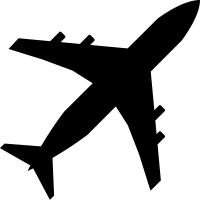
\includegraphics[width=1.5cm]{figs/airplane.png}}\quad
%		\subfloat{
%		
\includegraphics[width=1.5cm]{figs/car.png}}\quad
%		\subfloat{
%		
\includegraphics[width=1.5cm]{figs/train.png}}\quad
%		\subfloat{
%		
\includegraphics[width=1.5cm]{figs/medical.png}}
%	\end{figure}
%
%	\begin{alertblock}{Current industrial trends}<2->
%		\begin{itemize}
%			\item Reduce size, weight, power consumption, costs, heat, \dots
%			\item Integrate software components into a single 
%			\textbf{multi-core architecture}.
%			\item Deliver more functionalities.
%		\end{itemize}
%	\end{alertblock}
%\end{frame}
%
%%------------------------------------------------------------------------------
%\part{Design of Mixed-criticality and data-driven safety-critical systems}
%%------------------------------------------------------------------------------
%
%\begin{frame}[noframenumbering]
%		\frametitle{Part I: Design of Mixed-criticality and data-driven 
%		safety-critical systems}
%		\tableofcontents[hideothersubsections]
%\end{frame}
%
%%------------------------------------------------------------------------------
%\section{Logical correctness}
%%------------------------------------------------------------------------------
%
%\miniframeson
%\begin{frame}
%	\frametitle{Logical correctness: Data-driven models}
%	
%	\begin{itemize}
%		\item Models of Computation (MoC): data-flow graphs \&\\
%		Directed Acyclic Graphs (DAGs).
%		\item Many extensions to the initial Kahn Process Network model.
%		\begin{itemize}
%			\item Communication models (Synchronous Data-flow).
%			\item Functional properties can be proven,\\
%			\emph{e.g.} deadlock/starvation freedom, boundedness in memory.
%			\item Natural representation of data sharing and parallelism.
%			\item Time constraints.
%		\end{itemize}
%	\end{itemize}
%	
%	\begin{figure}
%		\vspace{-0.5cm}
%		\subfloat{
%			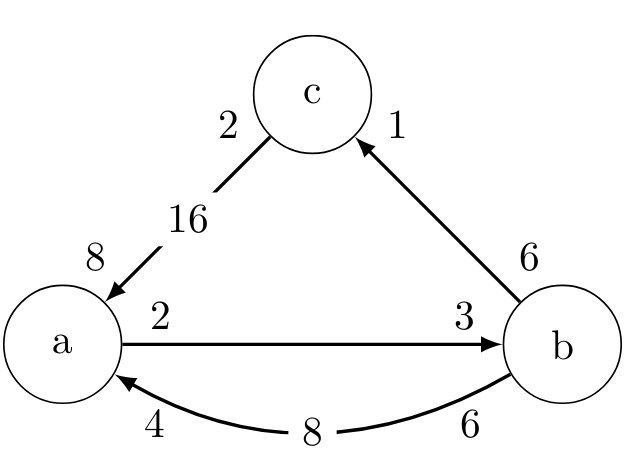
\includegraphics[width=3.5cm]{figs/sdfg.png}}\quad
%		\subfloat{
%			\raisebox{1.5em}{
%				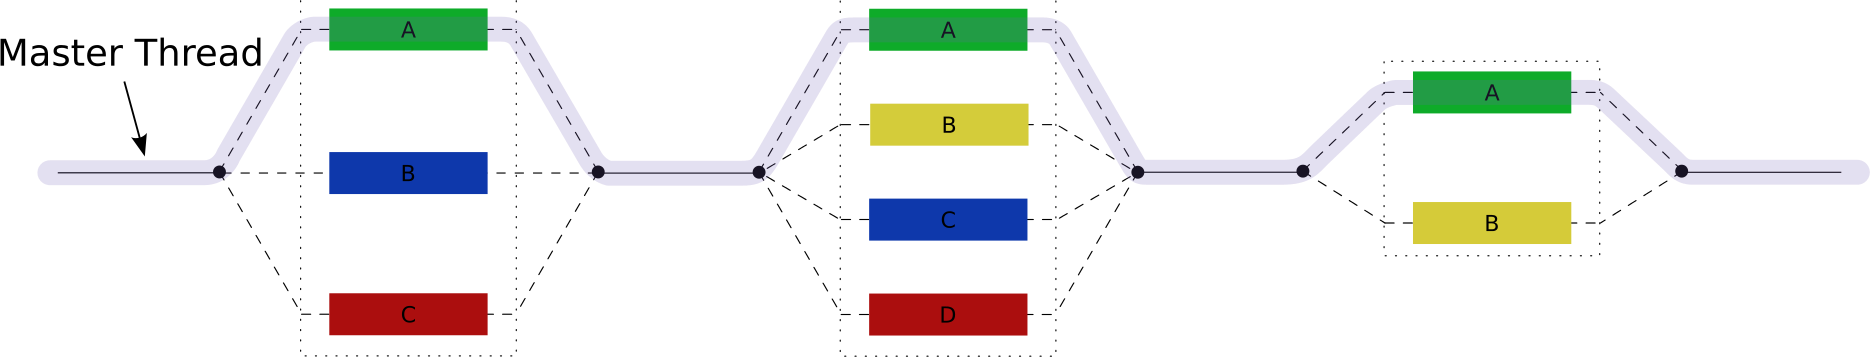
\includegraphics[width=6.5cm]{figs/Fork_join.png}}}
%	\end{figure}
%
%\end{frame}
%
%%------------------------------------------------------------------------------
%
%\begin{frame}
%	\frametitle{Logical correctness: MoC applicability in the industry}
%	
%	\begin{itemize}
%	\item Industrial tools based on these models\\
%	 (\emph{e.g.} Simulink, 
%	SCADE).
%		\begin{itemize}
%			\item Widely used in safety-critical control software,\\
%			\emph{e.g.} 
%			Flight Control Systems.
%			\item Code generation, automatic deployment into architectures.
%		\end{itemize}
%		
%		\begin{figure}
%			\centering
%			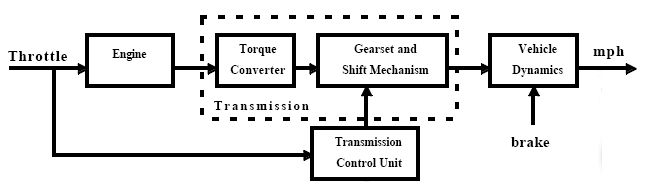
\includegraphics[width=10cm]{figs/simulink.png}
%		\end{figure}
%	\end{itemize}
%	\pnote{Awesome note}
%\end{frame}
%
%%------------------------------------------------------------------------------
%\section{Time correctness}
%%------------------------------------------------------------------------------
%
%
%\begin{frame}
%\frametitle{Time correctness: Real-time systems}
%	\begin{itemize}
%		\item \textbf{A correct output is an output on time.}
%
%		\item Real-time (RT) scheduling ensures temporal correctness.
%		\begin{itemize}
%			\item Tasks have deadlines ($D_i$), periods ($T_i$), timing budgets 
%			($C_i$).
%		\end{itemize}
%		\item \textbf{Schedulability}: allocate tasks into processors 
%		respecting deadlines and periods.
%	\end{itemize}
%
%	\begin{figure}
%		\centering
%		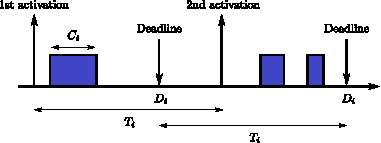
\includegraphics[width=9cm]{figs/rt_task.pdf}
%	\end{figure}
%	
%	\begin{itemize}
%		\item<2> RT systems dimensioned with Worst Case Execution Time (WCET).
%	\end{itemize}
%\end{frame}
%%------------------------------------------------------------------------------
%\begin{frame}
%\frametitle{Time correctness: Worst-Case Execution Time estimation}
%	\begin{figure}
%		\centering
%		\includegraphics<1|handout:0>[width=10cm]{figs/clo0.pdf}
%		\includegraphics<2|handout:0>[width=10cm]{figs/clo1.pdf}
%		\includegraphics<3|handout:0>[width=10cm]{figs/clo2.pdf}
%		\includegraphics<4>[width=10cm]{figs/clo.pdf}
%	\end{figure}
%
%	\begin{itemize}
%	\item Estimating the WCET: a difficult 
%	problem~\footfullcite{wilhelm2008worst}.
%		\begin{itemize}
%			\item<3-4> Various methods to obtain an estimate.
%			\item<4> Obtain a safe upper-bound.
%			\item<4> Task rarely executes until its WCET.
%
%			\item<4> Multi-core architectures hardly predictable.
%		\end{itemize}
%	\end{itemize}
%\end{frame}
%%------------------------------------------------------------------------------
%\section{Mixed-Criticality model}
%%------------------------------------------------------------------------------
%\begin{frame}
%\frametitle{Mixed-Criticality (MC) model: system's execution}
%	\begin{enumerate}
%		
%		\item Incorporate tasks with different criticality levels: HI and LO.
%		\item Execution modes:
%		\begin{itemize}
%			\item LO-criticality mode: HI tasks + LO tasks.
%			\item HI-criticality mode: HI tasks $\rightarrow$ 
%			LO tasks degraded.
%		\end{itemize}
%		\item Different timing budgets~\footcite{vestal2007preemptive}.
%		\begin{itemize}
%			\item $C_i(LO)$: Max. observed execution time (system designers).
%			\item $C_i(HI)$: Upper-bounded execution time (static analysis).
%		\end{itemize}
%		\item System switches to HI-criticality mode when needed.
%	\end{enumerate}
%
%	\pnote{MORE Awesome note}
%	
%%	\begin{figure}
%%		\centering
%%		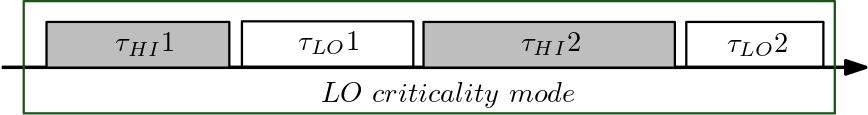
\includegraphics[width=9cm]{figs/mxsched.png}
%%	\end{figure}
%%	\begin{figure}
%%		\centering
%%		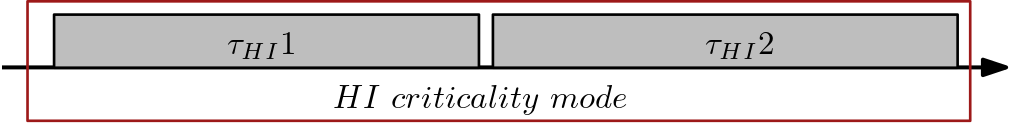
\includegraphics[width=9cm]{figs/mxschedhi.png}
%%	\end{figure}
%
%\end{frame}
%
%%------------------------------------------------------------------------------
%
%\begin{frame}
%	\frametitle{MC model: Schedulability with mode transitions}
%	\begin{itemize}
%		\item Example: HI tasks: $\tau_1, \tau_3$. LO tasks: $\tau_2, \tau_4$.
%		\item Assuming the following scheduling.
%		\item<2> Timing Failure Event (TFE) $\rightarrow$ Mode transitions 
%		$\rightarrow$ \textbf{potential deadline misses}.
%	\end{itemize}
%	
%	\begin{figure}
%		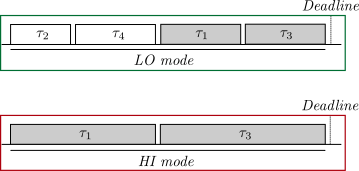
\includegraphics[width=7cm]{figs/mode_transition0}
%	\end{figure}
%	
%	\begin{figure}
%		\hspace{1cm}
%		\includegraphics<2>[width=8.2cm]{figs/mode_transition}
%	\end{figure}
%
%\end{frame}
%
%%------------------------------------------------------------------------------
%
%\begin{frame}
%	\frametitle{MC model: Availability of LO-criticality tasks}
%	\begin{itemize}
%		\item Example: same task set as before.
%	\end{itemize}
%	\begin{figure}
%		\subfloat{
%		\includegraphics<1->[width=7cm]{figs/avail_motiv0.pdf}}
%	
%		\subfloat{
%		\includegraphics<2->[width=7cm]{figs/avail_motiv1.pdf}}
%	\end{figure}
%
%	\begin{itemize}
%		\item<2-> Schedulability \textit{but} LO-criticality tasks discarded:
%		some services are no longer delivered.
%	\end{itemize}
%
%\end{frame}
%
%
%
%
%%------------------------------------------------------------------------------
%\miniframesoff
%\begin{frame}
%	\frametitle{General research objectives}
%	
%	\begin{itemize}
%		\item \textbf{Objective 1}: Demonstrate that safety-critical 
%		systems can be MC, data-driven and efficiently execute in multi-core 
%		architectures.
%		\item \textbf{Objective 2}: Demonstrate that MC systems can deliver an 
%		acceptable availability rate.
%	\end{itemize}
%\end{frame}
%
%
%
%%------------------------------------------------------------------------------
%\section{System hypotheses}
%%------------------------------------------------------------------------------
%\miniframeson
%\begin{frame}
%	\frametitle{System hypotheses}
%	
%	\begin{table}[h]
%		\centering
%		\begin{tabular}{|l|l|}
%			\hline
%			\multicolumn{2}{|c|}{\textbf{Data-dependencies}}               \\ 
%			\hline
%			Graph               & Directed acyclic graphs.                 \\ 
%			\hline
%			Vertices            & Real-time tasks.                         \\ 
%			\hline
%			Edges               & Precedence constraints.                  \\ 
%			\hline
%			\multicolumn{2}{|c|}{\textbf{Real-time}}                       \\ 
%			\hline
%			Execution time      & Tasks use all their timing budget.       \\ 
%			\hline
%			Period              & Tasks are periodic.                      \\ 
%			\hline
%			Deadline            & Constrained or implicit. \\ 
%			\hline
%			\multicolumn{2}{|c|}{\textbf{Architecture}}                    \\ 
%			\hline
%			Processors          & Multi-core 
%			homogeneous.                             \\ 
%			\hline
%			Communication costs & Considered in tasks execution time.      \\ 
%			\hline
%			\multicolumn{2}{|c|}{\textbf{Mixed-criticality}}               \\ 
%			\hline
%			Criticality levels  & Two or more criticality levels.          \\ 
%			\hline
%			Timing budgets      & Monotonically increasing.                \\ 
%			\hline
%			Degradation         & Discarding lowest-criticality tasks.     \\ 
%			\hline
%		\end{tabular}
%	\end{table}
%	
%	
%%	A Mixed-Criticality System (MCS) is a tuple $\mathcal{S} = (\Pi, 
%%	\mathcal{CL}, \mathcal{G})$.
%%	\begin{itemize}
%%		\item $\Pi$: \emph{homogeneous} architecture. 
%%		\begin{itemize}
%%			\item $|\Pi| = m$ number of 
%%			cores.
%%			\item Cores communicate through an interconnect bus.
%%		\end{itemize}
%%		\item $\mathcal{CL} = \{\chi_1, \dots, \chi_n \}$ set of criticality 
%%		levels.
%%		\begin{itemize}
%%			\item A priority ordering $\prec$ can be defined for any $(\chi_i, 
%%			\chi_j) \in \mathcal{CL}^2$.
%%		\end{itemize}
%%		\item $\mathcal{G}$ set of DAGs executing in the system.
%%	\end{itemize}
%\end{frame}
%
%%------------------------------------------------------------------------------
%\section {Applications description}
%%------------------------------------------------------------------------------
%
%\begin{frame}
%	\frametitle{Mixed-Criticality Directed Acyclic Graphs}
%	\begin{columns}
%		\begin{column}{0.45\textwidth}
%			MC-DAG $G_j \in \mathcal{G}$.\\
%			$G_j=(V_j, E_j, D_j, T_j)$.
%			\begin{itemize}
%				\item<2-> $V_j$ set of vertices.
%				\item<3-> $E_j \subseteq (V_j \times V_j)$ set of edges.
%				\item<4-> $D_j$ deadline.
%				\item<5-> $T_j$ period.
%			\end{itemize}
%			\only<6->{Vertex $\tau_i = (\chi_i, 
%			C_i(\chi_1), \dots, C_i(\chi_\ell))$}
%			\begin{itemize}
%				\item<6-> $\chi_i \in \mathcal{CL}$. criticality level of the 
%				task.
%				\item<7-> $C_i(\chi_1), \dots, C_i(\chi_\ell)$ timing 
%				budgets.
%			\end{itemize}
%		\end{column}
%		\begin{column}{0.6\textwidth}
%			\begin{figure}
%				\includegraphics<1|handout:0>[width=6cm]{figs/multidag_lo0.pdf}
%				\includegraphics<2|handout:0>[width=6cm]{figs/multidag_lo1.pdf}
%				\includegraphics<3|handout:0>[width=6cm]{figs/multidag_lo2.pdf}
%				\includegraphics<4|handout:0>[width=6cm]{figs/multidag_lo3.pdf}
%				\includegraphics<5|handout:0>[width=6cm]{figs/multidag_lo4.pdf}
%				\includegraphics<6|handout:0>[width=6cm]{figs/multidag_lo5.pdf}
%				\includegraphics<7>[width=6cm]{figs/multidag_lo.pdf}
%			\end{figure}
%		\end{column}
%	\end{columns}
%\end{frame}
%
%%------------------------------------------------------------------------------
%\part{Scheduling MC-DAGs on multi-core architectures}
%%------------------------------------------------------------------------------
%
%\begin{frame}[noframenumbering]
%	\frametitle{Part II: Scheduling MC-DAGs on multi-core architectures}
%	\tableofcontents[hideothersubsections]
%\end{frame}
%
%%------------------------------------------------------------------------------
%\section{Problem: MC-DAG scheduling}
%%------------------------------------------------------------------------------
%\miniframeson
%\begin{frame}
%	\frametitle{Problem statement: multi-core DAG and MC schedulability}
%	\centering
%	\textbf{Objective 1}: Demonstrate that safety-critical 	systems can be MC, 
%	data-driven and efficiently execute in multi-core 
%	architectures.
%	\begin{itemize}
%		\item<2-> DAG scheduling: \textbf{NP-complete} 
%		problem~\footfullcite{Kwok1999}.
%		\begin{itemize}
%			\item<2-> List Scheduling, RT schedulers with response time analysis
%			\item<2-> \textbf{No variations in timing budgets} in the 
%			literature.
%			\item<2-> \textbf{No mode transitions for the system}.
%		\end{itemize}
%		\item<3-> MC scheduling is intractable: \textbf{NP-hard} 
%		problem~\footfullcite{baruah2009mixed}.
%		\begin{itemize}
%			\item<3-> Most schedulers (\emph{e.g.} EDF-vd, MC-Fluid) for 
%			\textbf{independent} MC task sets.
%			\item<3-> When precedence constraints are considered, 
%			\textbf{systems 
%			are overdimensioned.}
%		\end{itemize}
%
%	\end{itemize}
%
%	\begin{block}{}<4->
%		\textbf{Conclusion}: we need new efficient scheduling methods.
%	\end{block}
%	
%\end{frame}
%
%
%%------------------------------------------------------------------------------
%
%\begin{frame}
%	\frametitle{Problem statement: multi-core DAG and MC schedulability}
%	
%	\begin{itemize}
%		
%		\item\textbf{Problem S1}: Schedulability of MC-DAGs on multi-cores.
%		\item \textbf{Problem S2}: Improving acceptance rate for single MC-DAG 
%		scheduling.
%		\item \textbf{Problem S3}: Improving resource utilization for 
%		multi-periodic MC-DAGs.
%		\item \textbf{Problem S4}: Generalization to multiple criticality 
%		levels.
%	\end{itemize}
%\end{frame}
%
%
%%------------------------------------------------------------------------------
%\section {MC-correctness}
%%------------------------------------------------------------------------------
%
%\begin{frame}
%	\frametitle{MC-correctness for DAGs in multi-cores}
%
%	\begin{definition}
%	\textbf{MC-correctness}\footfullcite{baruah2016federated} (for 
%	dual-criticality systems).
%		\begin{enumerate}
%			\item \textbf{Condition LO-mode}: If no vertex of any MC-DAG 
%			executes beyond its $C_i(LO)$ then all the vertices complete 
%			execution by their deadlines.
%			\item \textbf{Condition HI-mode}: If no vertex of any MC-DAG 
%			executes beyond its $C_i(HI)$ then all the vertices designated as 
%			being of HI-criticality complete their execution by their deadlines.
%		\end{enumerate}
%	\label{def:mccorrect}
%	\end{definition}
%
%	\begin{exampleblock}{Ensuring \textbf{Cond. LO-mode}}<2>
%		Define a \textit{correct} scheduling for the LO-criticality mode.
%	\end{exampleblock}
%\end{frame}
%
%
%
%%------------------------------------------------------------------------------
%
%\begin{frame}
%	\frametitle{Ensuring \textbf{Cond. HI-mode}: Safe Transition Property}
%	\begin{itemize}
%		\item \emph{Intuition}: At any instant $t$, HI task execution time 
%		given in LO mode at least equal to execution time given in HI mode.
%		\item $\psi_i^{\chi}(t_1, t_2)$: cumulative execution time given to 
%		task $\tau_i$.
%	\end{itemize}
%
%	\begin{figure}
%		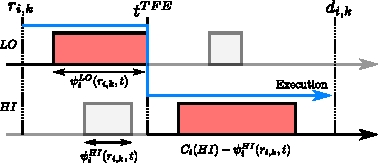
\includegraphics[width=7cm]{figs/proof_case3.pdf}
%	\end{figure}
%
%	\begin{exampleblock}{Safe Transition Property}
%		\begin{equation}
%			\psi_i^{LO}(r_{i,k}, t) < C_i(LO) \implies \psi_i^{LO}(r_{i,k}, t) 
%			\geq \psi_i^{HI}(r_{i,k},t).
%			\label{eq:condswitch}
%		\end{equation}
%	\end{exampleblock}
%\end{frame}
%
%%------------------------------------------------------------------------------
%
%\begin{frame}
%	\frametitle{Meta-heuristic for MC-DAG scheduling}
%	
%	\begin{itemize}
%		\item Solve the complex scheduling problem \emph{off-line} thanks to 
%		\textbf{scheduling tables}:
%		\begin{itemize}
%			\item Easier to verify and have certified.
%			\item Easier to calculate $\psi_i^\chi$, enforce \textbf{Safe 
%			Trans. Prop.}
%		\end{itemize}
%	\end{itemize}
%
%	\begin{exampleblock}{\textsc{Mh-McDag}}
%		\begin{itemize}
%			\item Compute scheduling table in HI-criticality mode.
%			\item Compute scheduling table in LO-criticality mode,\\
%			enforcing \textbf{Safe Trans. Prop.}
%		\end{itemize}
%		Produces \textbf{MC-correct} schedulers for MC-DAGs.
%	\end{exampleblock}
%
%	\begin{itemize}
%		\item<2> \textsc{Mh-McDag} $\rightarrow$ \textbf{Problem S1} 
%		$\checkmark$.
%	\end{itemize}
%\end{frame}
%
%
%
%%------------------------------------------------------------------------------
%\section{Relaxation of HI tasks}
%%------------------------------------------------------------------------------
%
%\begin{frame}
%	\frametitle{Constrained HI-criticality tasks execution (1/2)}
%	\setcounter{subfigure}{0}
%	
%
%	\begin{itemize}
%		\item Existing approach based on List 
%		Scheduling~\footfullcite{baruah2013implementing}.
%		\item Computes two \emph{independent} priority 
%		orderings.
%		\item Two scheduling tables are produced.
%		\item HI-criticality scheduled ASAP.
%		\begin{itemize}
%			\item Ensures safe mode transitions.
%		\end{itemize}
%		\item Implicit implementation of \textsc{Mh-McDag}.
%	\end{itemize}
%
%\end{frame}
%
%%------------------------------------------------------------------------------
%
%\begin{frame}
%	\frametitle{Constrained HI-criticality tasks execution (2/2)}
%	
%		\begin{figure}
%		\vspace{-0.5cm}
%		\begin{tabular}{cc}
%			\adjustbox{valign=c}{\subfloat[Single MC-DAG system]{
%					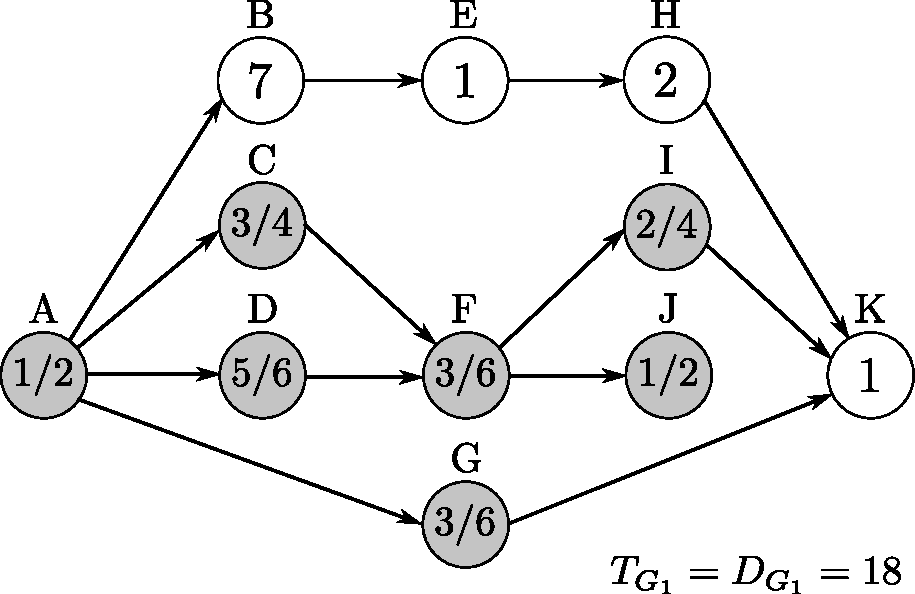
\includegraphics[width=5cm]{figs/ada_lo.pdf}
%				}
%			}
%			
%			&
%			
%			\adjustbox{valign=c}{\begin{tabular}{@{}c@{}}
%					\subfloat[$S_{HI}$ scheduling 
%					table]{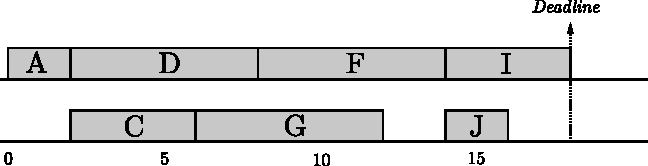
\includegraphics[width=5cm]{figs/ada_baruah_shi.pdf}
%						\label{subfig:sched_baruah_shi}}\\
%					
%					\subfloat[$S_{LO}$ scheduling 
%					table]{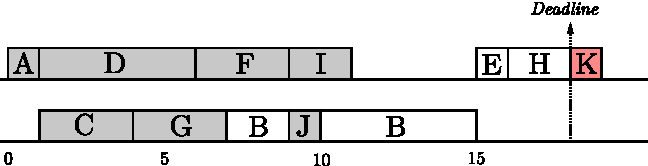
\includegraphics[width=5cm]{figs/ada_baruah_slo.pdf}
%						\label{subfig:sched_baruah_slo}}
%					\label{fig:sched_baruah_single}
%			\end{tabular}}
%		\end{tabular}
%		
%	\end{figure}
%	
%	\begin{figure}
%		\centering
%		
%	\end{figure}
%	
%	\begin{alertblock}{}
%		\begin{itemize}
%			\item Non-schedulable under 18 TUs and 2 cores.
%			\item Task $B$ activated after 1 TU, constantly preempted.
%			\begin{itemize}
%				\item Response time of LO-criticality tasks affected.
%			\end{itemize}
%		\end{itemize}
%	\end{alertblock}
%
%\end{frame}
%
%%------------------------------------------------------------------------------
%
%\begin{frame}
%	\frametitle{Relaxation of HI-criticality tasks (1/2)}
%	\begin{itemize}
%
%		\item \emph{ALAP execution} of HI tasks in HI mode.
%		\begin{itemize}
%			\item Transform the graph into its \emph{dual} and perform the 
%			scheduling.
%		\end{itemize}
%
%
%	\end{itemize}
%
%
%	\begin{figure}
%	\vspace{-0.5cm}
%	\begin{tabular}{cc}
%		\adjustbox{valign=c}{\subfloat{
%				\includegraphics<1|handout:0>[width=5cm]{figs/ada_hi_star0.pdf}
%				\includegraphics<2->[width=5cm]{figs/ada_hi_star.pdf}
%			}
%		}
%		
%		&
%		
%		\adjustbox{valign=c}{\begin{tabular}{@{}c@{}}
%			\subfloat{
%				\includegraphics<3->[width=5cm]{figs/ada_us_shi0.pdf}
%			} \\
%		
%			\subfloat{
%				\includegraphics<4->[width=5cm]{figs/ada_us_shi.pdf}
%			}
%		\end{tabular}}
%	\end{tabular}
%	
%	\end{figure}
%
%
%	
%\end{frame}
%
%\begin{frame}
%	\frametitle{Relaxation of HI-criticality tasks (2/2)}
%	\begin{itemize}
%		\item \emph{Precise prioritization}: HI-criticality tasks only 
%		preempt to respect \textbf{Safe Trans. Prop.}
%	\end{itemize}
%	
%	\setcounter{subfigure}{0}
%	
%	
%	\begin{figure}
%		\vspace{-0.5cm}
%		\begin{tabular}{cc}
%			\adjustbox{valign=c}{\subfloat[Single MC-DAG system]{
%					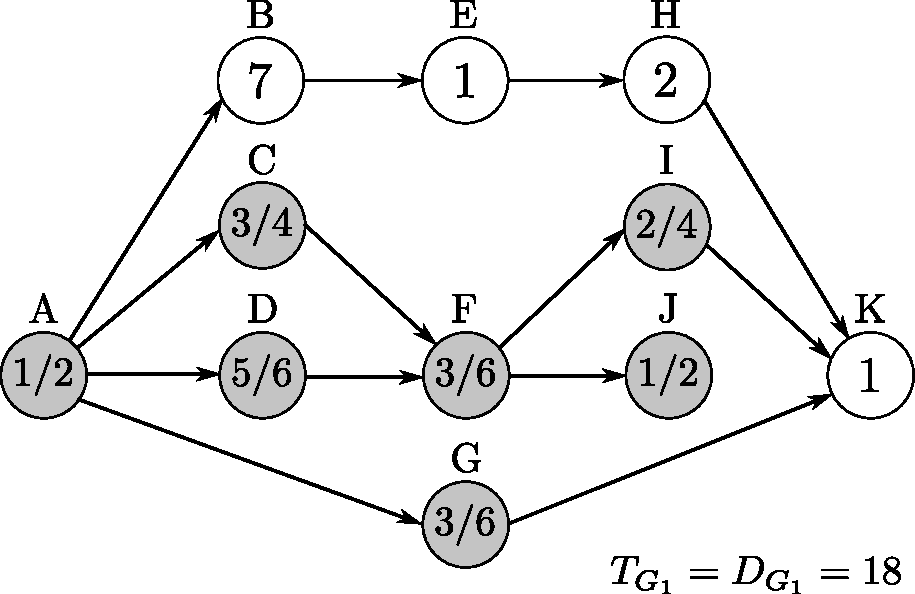
\includegraphics[width=5cm]{figs/ada_lo.pdf}
%				}
%			}
%			
%			&
%			
%			\adjustbox{valign=c}{\begin{tabular}{@{}c@{}}
%					\subfloat[ALAP scheduling in HI mode]{
%						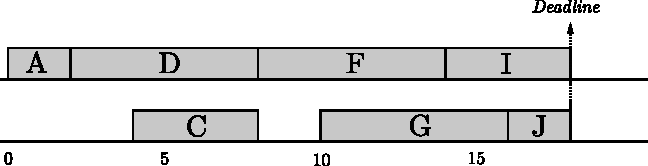
\includegraphics[width=5cm]{figs/ada_us_shi.pdf}} \\
%					
%					\subfloat[ASAP scheduling in LO mode]{
%						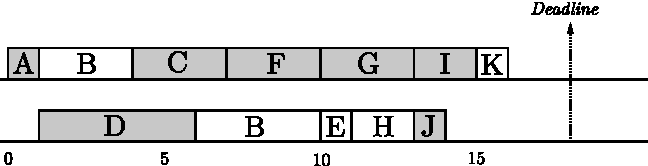
\includegraphics[width=5cm]{figs/ada_us_slo.pdf}}
%			\end{tabular}}
%		\end{tabular}
%		
%	\end{figure}
%
%	
%	\begin{itemize}
%		\item LO-criticality tasks have more usable timeslots.
%		\item Relaxation of HI tasks $\rightarrow$ 		\textbf{Problem S2} 
%		$\checkmark$
%	\end{itemize}
%\end{frame}
%
%%------------------------------------------------------------------------------
%\section {Global multi-periodic scheduling}
%%------------------------------------------------------------------------------
%\newcommand{\light}[1]{\textcolor{gray}{#1}}
%
%\begin{frame}
%	\frametitle{Multi-periodic MC-DAG}
%	Existing approach~\footfullcite{baruah2016federated}:
%	\begin{itemize}
%		\item Federated: MC-DAGs are categorized as \emph{light} or 
%		\emph{heavy}.
%		\begin{itemize}
%			\item Light DAGs transformed into sequential tasks.
%			\item Heavy DAGs, $U_{max} > 1$, more than 1 core to execute.
%		\end{itemize}
%		\item Clusters to schedule sporadic heavy MC-DAGs.
%		\item Scheduling tables are computed for each cluster.
%		\item \textbf{Poor resource usage}: vertices of different MC-DAGs do 
%		not share cores.
%	\end{itemize}
%\end{frame}
%
%%------------------------------------------------------------------------------
%
%\begin{frame}
%	\frametitle{An example of multi-periodic MCS}
%	\setcounter{subfigure}{0}
%
%	\begin{figure}
%		\vspace{-0.7cm}
%		\begin{tabular}{cc}
%			\adjustbox{valign=c}{\subfloat[Multi-periodic MCS]{
%					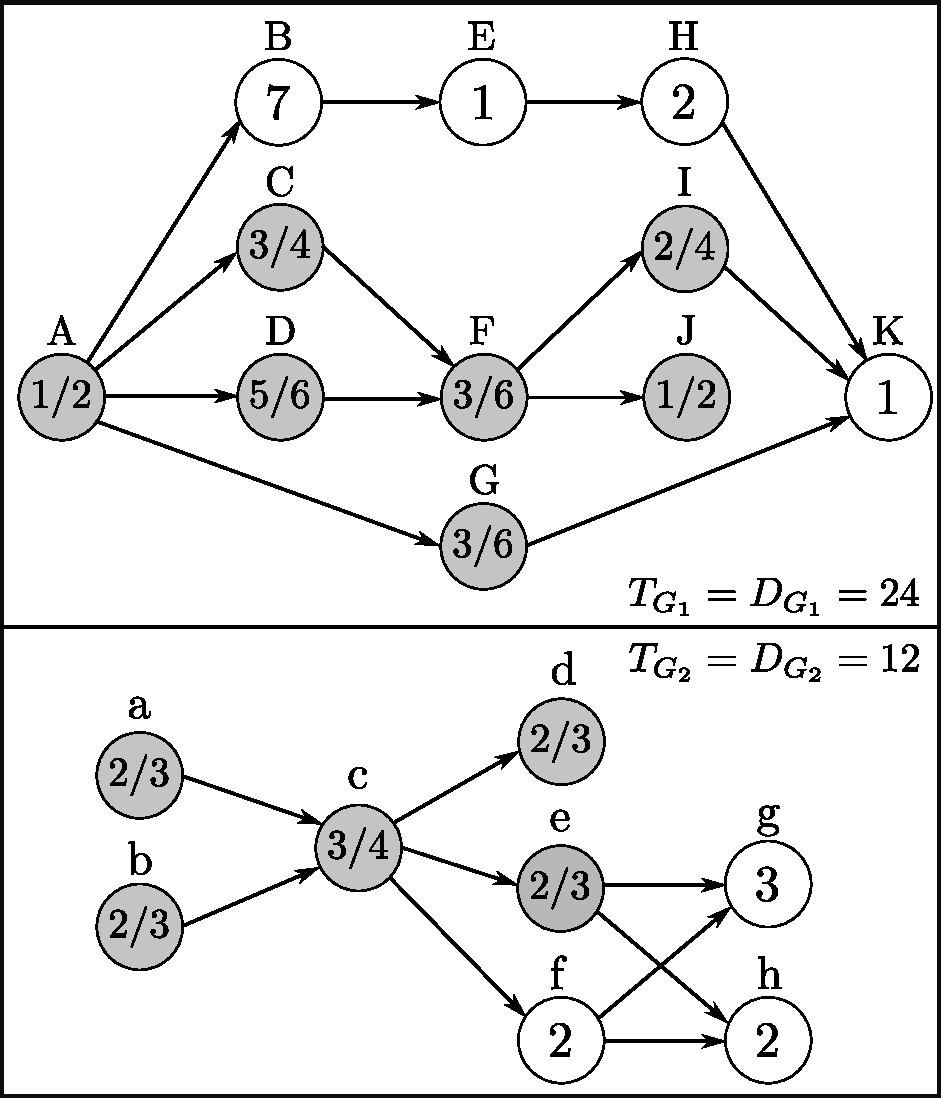
\includegraphics[width=5cm]{figs/multidag_lo.pdf}}}
%			
%			&
%			
%			\adjustbox{valign=c}{\begin{tabular}{@{}c@{}}
%					\subfloat[Federated approach: HI-criticality mode]{
%						
%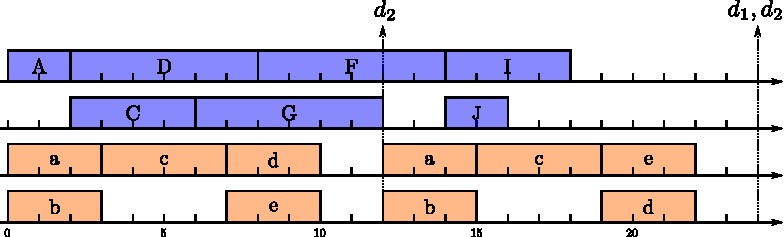
\includegraphics[width=5.5cm]{figs/multiple_shi_federated.pdf}
%						\label{subfig:sched_federated_shi}
%					}\\
%					
%					\subfloat[Federated approach: LO-criticality mode]{
%						
%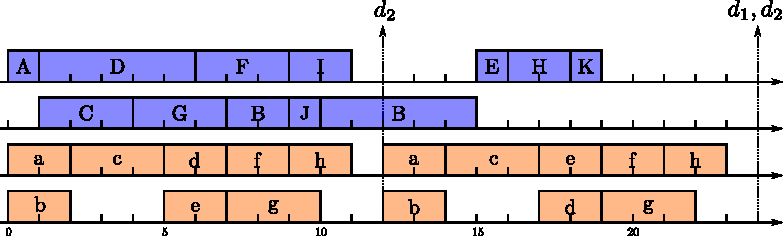
\includegraphics[width=5.5cm]{figs/multiple_slo_federated.pdf}
%						\label{subfig:sched_federated_slo}
%					}
%			\end{tabular}}
%		\end{tabular}
%	\end{figure}
%
%	\begin{itemize}
%		\item At least 2 clusters of 2 cores.
%		\item Max utilization of the system is inferior to 3.
%	\end{itemize}
%\end{frame}
%
%
%%------------------------------------------------------------------------------
%
%\begin{frame}
%	\frametitle{Global approach for multi-periodic MC-DAGs}
%
%	\begin{itemize}
%		\item \textbf{Safe Trans. Prop.} usable for the multi-period case.
%		\item Various implementations thanks to \textsc{Mh-McDag} 
%		\textbf{genericity}.
%	\end{itemize}
%
%	\begin{table}
%		\begin{tabular}{|c|c|}
%			\hline
%			\textbf{Implementation} & \textbf{Prio. 
%			Ordering}                                           \\ \hline
%			G-EDF                   & $D_{i,k}^\chi = d_{i,k} - 
%			CP_i^{\chi}$                            \\ \hline
%			G-LLF                   & $L_{i,k}^\chi (t) = d_{i,k} - t - 
%			(CP_i^{\chi} + R_{i,k}^{\chi})$ \\ \hline
%			Hybrid                  & G-EDF HI mode/G-LLF LO 
%			mode                                      \\ \hline
%		\end{tabular}
%	\end{table}
%%
%%	\begin{itemize}
%%		\item $d_{i,k}$ deadline of the $k$-th activation of the MC-DAG.
%%		\item $CP_i^{\chi}$ critical path to the vertex.
%%		\item $t$ current time slot.
%%		\item $R_{i,k}^{\chi}$ remaining execution time.
%%		\begin{itemize}
%%			\item Initialized with $C_i(LO)$ or $C_i(HI)$.
%%		\end{itemize}
%%	\end{itemize}
%
%\end{frame}
%
%
%%------------------------------------------------------------------------------
%
%\begin{frame}
%	\frametitle{\textsc{G-alap} scheduling tables}
%	\begin{columns}
%		\begin{column}{.5\textwidth}
%			\begin{figure}
%				\centering
%				\subfloat[\textsc{G-alap-edf} HI mode]{
%					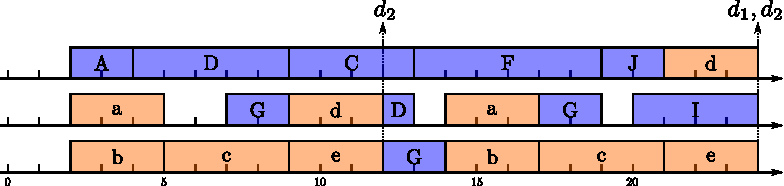
\includegraphics[width=5.5cm]{figs/multiple_shi_edf.pdf}
%					\label{subfig:multiple_gedf_hi}
%				}
%				
%				\subfloat[\textsc{G-alap-edf} LO mode]{
%					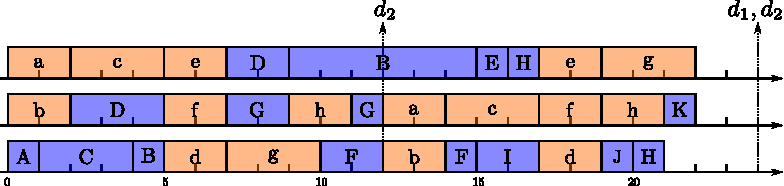
\includegraphics[width=5.5cm]{figs/multiple_slo_edf.pdf}
%					\label{subfig:multiple_gedf_lo}
%				}
%			\end{figure}
%		\end{column}
%	
%		\begin{column}{.5\textwidth}
%			\begin{figure}
%				
%				\subfloat[\textsc{G-alap-llf} HI mode]{
%					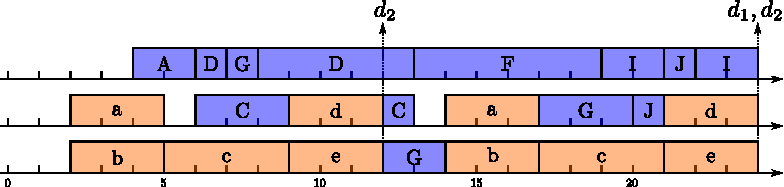
\includegraphics[width=5.5cm]{figs/multiple_shi.pdf}
%					\label{subfig:multiple_gllf_hi}
%				}
%				
%				\subfloat[\textsc{G-alap-llf} LO mode]{
%					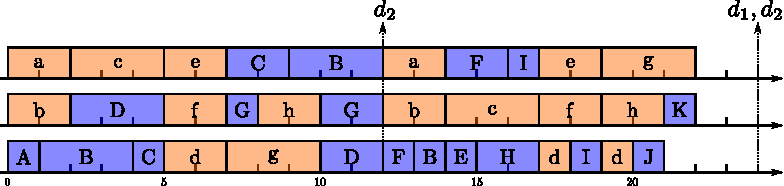
\includegraphics[width=5.5cm]{figs/multiple_slo.pdf}		
%						
%					\label{fig:multiple_slo}
%				}
%				
%			\end{figure}
%		\end{column}
%	\end{columns}
%	
%	
%	\begin{itemize}
%		\item MC-correct scheduling tables found with \textbf{only 3 cores}.
%		\item Efficient multi-periodic MC-DAG scheduling\\
%		$\rightarrow$ \textbf{Problem S3} $\checkmark$.
%	\end{itemize}
%\end{frame}
%
%%------------------------------------------------------------------------------
%\section {Multiple criticality levels}
%%------------------------------------------------------------------------------
%
%%------------------------------------------------------------------------------
%
%\begin{frame}
%	\frametitle{Generalization of MC-correctness}
%	
%	\begin{itemize}
%		\item MCS with criticality levels $\mathcal{CL} = \{ \chi_1, \dots, 
%		\chi_\ell, \dots, \chi_n \}$,\\
%		safety-critical standards define more than two criticality levels.
%	\end{itemize}
%	
%	\begin{definition}
%        \textbf{Generalized MC-correctness} - A generalized MC-correct 
%        scheduling is one that guarantees:
%		\begin{enumerate}
%			\item  If all vertices of any MC-DAG execute within their 
%			$C_i(\chi_1)$, then all vertices complete their execution by the 
%			deadlines; and 
%			\item If no vertex of any MC-DAG executes 
%			beyond its $C_i(\chi_\ell)$, then all vertices that are designed as 
%			being of $\chi_\ell$-criticality complete their execution by their 
%			deadlines.
%		\end{enumerate}
%	\label{def:general_mccorrect}
%	\end{definition}
%\end{frame}
%
%%------------------------------------------------------------------------------
%
%\begin{frame}
%	\frametitle{Generalized Safe Transition Property}
%	
%	\begin{itemize}
% 		\item \textbf{Problem}: More scheduling tables to compute.
%	\end{itemize}
%	
%	\begin{exampleblock}{Generalized Safe Transition Property}
%        \begin{equation}
%			\psi_i^{\chi_\ell} (r_{i,k}, t) < C_i(\chi_\ell) \implies 
%			\psi_i^{\chi_\ell}(r_{i,k}, t) \geq 
%			\psi_i^{\chi_{\ell+1}}(r_{i,k},t).
%			\label{eq:start_n_mode_lo}
%		\end{equation}
%	\end{exampleblock}
%
%	\begin{exampleblock}{\textsc{N-Mh-McDag}}
%		Meta-heuristic for multi-periodic MC-DAG scheduling with an 
%		arbitrary number of criticality levels.
%		\begin{enumerate}
%			\item Schedule the MC system in descending order.
%			\item While scheduling criticality modes that are not the 
%			highest-criticality mode, enforce \textbf{Gen. Safe Trans. Prop.}
%		\end{enumerate}
%	\end{exampleblock}
%\end{frame}
%
%%------------------------------------------------------------------------------
%
%\begin{frame}
%	\frametitle{Safe transition property in the dual graph}
%	
%	\begin{itemize}
%		\item \textbf{Problem}: Keep relaxation in the generalized case,
%		scheduling on the dual graph.
%	\end{itemize}
%
%	\begin{figure}
%		
%\includegraphics<1|handout:0>[width=\textwidth]{figs/generalization_ill0.pdf}
%		\includegraphics<2->[width=\textwidth]{figs/generalization_ill.pdf}
%	\end{figure}
%
%	
%	\begin{block}<2->{Dual Graph Generalized Safe Transition Property}
%		\begin{equation}
%		\psi_i^{\chi_{\ell+1}}(r_{i,k}',t') \leq C_i(\chi_{\ell+1}) - 
%		C_i(\chi_\ell)  \implies \psi_i^{\chi_\ell}(r_{i,k}',t') = 0.
%		\end{equation}
%	\end{block}
%	
%%	\begin{theorem}
%%        Respecting \textbf{Dual Graph Generalized Safe Transition Property} 
%%on 
%%        the scheduling of the dual MC-DAGs in all criticality modes is 
%%        equivalent to respecting \textbf{Gen. Safe Trans. Prop.} on the 
%%normal 
%%        MC-DAGs.
%%	\end{theorem}
%
%	\begin{itemize}
%		\item<3> Recursively defined a generalized meta-heuristic for MC-DAGs 
%		$\rightarrow$ \textbf{Problem S4} $\checkmark$.
%	\end{itemize}
%\end{frame}
%
%
%%------------------------------------------------------------------------------
%% \subsection {Conclusion on MC-DAG scheduling}
%%------------------------------------------------------------------------------
%
%\begin{frame}
%	\frametitle{Conclusions on multi-core MC-DAG scheduling}
%	
%	\begin{itemize}
%		\item Solved the complex problem of MC-DAG scheduling on multi-cores.
%		\item Characterized a sufficient property to have safe mode 
%		transitions.
%		\item Defined a meta-heuristic to schedule MC-DAGs.
%		\begin{itemize}
%			\item Many implementations can be derived.
%		\end{itemize}
%		\item Improved schedulability and resource usage:
%		\begin{itemize}
%			\item  Relaxed HI-criticality tasks execution.
%			\item Global execution for multi-periodic MC-DAGs.
%		\end{itemize}
%		\item Generalization to an arbitrary number of criticality levels.
%	\end{itemize}
%\end{frame}
%
%
%%------------------------------------------------------------------------------
%\part{MC-DAG framework and benchmarks}
%%------------------------------------------------------------------------------
%
%\begin{frame}[noframenumbering]
%	\frametitle{Part III: MC-DAG framework and benchmarks}
%	\tableofcontents[hideothersubsections]
%\end{frame}
%
%
%%------------------------------------------------------------------------------
%\section {Problem: experimental environment}
%%------------------------------------------------------------------------------
%
%\miniframeson
%\begin{frame}
%	\frametitle{Problem statement: obtaining an experimental environment}
%	
%	\begin{itemize}
%		\item \textbf{Problem E1}: Test the performance of our scheduling 
%		algorithms.
%		\item \textbf{Problem E2}: Have an unbiased environment for profiling 
%		and testing.
%	\end{itemize}
%\end{frame}
%
%%------------------------------------------------------------------------------
%\section {Unbiased generation tool}
%%------------------------------------------------------------------------------
%
%
%\begin{frame}
%	\frametitle{Unbiased generation tool}		
%		\begin{itemize}
%			\item Integrate concepts of different communities.
%			\begin{itemize}
%				\item Avoid particular DAG shapes: create vertices using 
%				layers~\footfullcite{tobita2002standard}.
%				\item Distribute system utilization 
%				uniformly~\footfullcite{bini2005measuring}.
%			\end{itemize}
%			\item Many parameters need to be taken into account.
%			\begin{itemize}
%				\item Utilization of the system.
%				\item Number of MC-DAGs.
%				\item Number of vertices.
%				\item Probability to have an edge.
%				\item Ratio HI/LO-criticality tasks.
%			\end{itemize}
%			\item Integration into an open-source framework~\footnote{MC-DAG 
%			framework - \url{https://github.com/robertoxmed/MC-DAG}}.
%		\end{itemize}
%\end{frame}
%
%%------------------------------------------------------------------------------
%
%\begin{frame}
%	\frametitle{Unbiased generation algorithm}
%	
%	\begin{columns}
%		\begin{column}{.6\textwidth}
%			\begin{exampleblock}{MC-DAG generator}
%				\begin{enumerate}
%					\item<1-> Distribute utilization.
%					\item<1-> Draw a random deadline.
%					\item<2-> For each criticality level:
%					\begin{itemize}
%						\item<3-> \textbf{\textit{Vertex generation phase}} by 
%						layers.
%						\item<4-> \textbf{\textit{Incorporation of edges}}
%						following a given probability.
%						\item<5-> \textbf{\textit{Reduction phase}} reach a 
%						reduction factor.
%					\end{itemize}
%				\end{enumerate}
%			\end{exampleblock}
%		\end{column}
%	
%		\begin{column}{0.4\textwidth}
%			\begin{figure}
%				\includegraphics<3|handout:0>[width=4.5cm]{figs/random_dag0.pdf}
%				\includegraphics<4|handout:0>[width=4.5cm]{figs/random_dag1.pdf}
%				\includegraphics<5|handout:0>[width=4.5cm]{figs/random_dag2.pdf}
%				\includegraphics<6->[width=4.5cm]{figs/random_dag.pdf}
%			\end{figure}
%		\end{column}
%	\end{columns}
%	
%	\begin{itemize}
%		\item<7-> Unbiased generation tool $\rightarrow$ \textbf{Problem E2} 
%		$\checkmark$.
%	\end{itemize}
%	
%\end{frame}
%
%%------------------------------------------------------------------------------
%\section {Experimental process}
%%------------------------------------------------------------------------------
%
%\begin{frame}
%	\frametitle{Experimental process}
%	
%	\begin{figure}
%		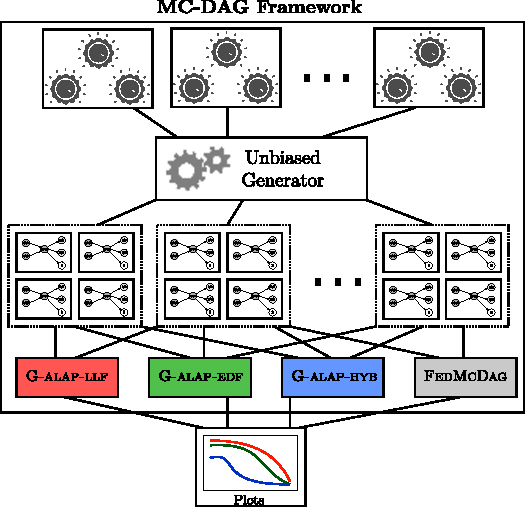
\includegraphics[width=8cm]{figs/expe_proc.pdf}
%	\end{figure}
%	
%%	\begin{itemize}
%%		\item \textbf{Setup}: Generated large number of MCS (1000 
%%		systems/configuration).
%%		\begin{itemize}
%%			\item Fixed number of cores and vertices.
%%			\item Vary the utilization of the system.
%%			\item Vary the number of MC-DAGs.
%%			\item Vary the density of the graph (edge probability).
%%			\item Measured the acceptance rate/number of preemptions for all 
%%			the scheduling algorithms of MC-DAGs.
%%		\end{itemize}
%%	\end{itemize}
%\end{frame}
%
%%------------------------------------------------------------------------------
%\section{Experimental results}
%%------------------------------------------------------------------------------
%
%%------------------------------------------------------------------------------
%\subsection{Acceptance rate}
%%------------------------------------------------------------------------------
%
%\begin{frame}
%	\frametitle{Acceptance rate: single MC-DAGs}
%	\setcounter{subfigure}{0}
%	\captionsetup[sub]{font=tiny,labelfont=tiny}
%	\begin{figure}
%		\vspace*{-0.5cm}
%		\subfloat[$m=4, |G|= 1,~ |V|= 50,~ e=20\%$]{
%			\begin{tikzpicture}[every mark/.append style={mark size=1.2pt}]
%			\begin{axis}[legend style={nodes={scale=0.7, transform shape}},
%			height=5.5cm, width=0.575\textwidth,
%			legend pos=south west,grid,
%			ytick={0, 0.1, ..., 1.1},
%			xtick={0.2, 0.3, ..., 1.1},
%			ymin=0]
%			
%			\addplot+[only marks,mark=star,red] table [x=Unorm, 
%			y=Lax50] {Results/l2/sched/c4/e20-d1.data};
%			\addplot+[only marks,mark=triangle,green!50!black] table [x=Unorm, 
%			y=Edf50] 
%			{Results/l2/sched/c4/e20-d1.data};
%			\addplot+[only marks,mark=diamond,blue] table [x=Unorm, y=Hyb50] 
%			{Results/l2/sched/c4/e20-d1.data};
%			\addplot+[only marks,mark=otimes,gray] table [x=Unorm, 
%			y=Baruah50] 
%			{Results/l2/sched/c4/e20-d1.data};
%			
%			\addplot [gray] 
%			gnuplot [raw gnuplot] { % "raw gnuplot" allows us to use arbitrary 
%				%gnuplot commands
%				f(x)=a*x^4+b*x^3+c*x^2+d*x+e;  % Define the function to fit
%				a=0.0001;
%				b=0.0001;
%				c=0.1;
%				d=0.1;
%				e=1;
%				fit f(x) 'Results/l2/sched/c4/e20-d1.data' using 1:6 via 
%				a,b,c,d,e; 
%				plot [x=0.25:1] f(x); % Specify the range to plot
%			};
%			\addplot [red] 
%			gnuplot [raw gnuplot] { % "raw gnuplot" allows us to use arbitrary 
%				%gnuplot commands
%				f(x)=a*x^4+b*x^3+c*x^2+d*x+e;  % Define the function to fit
%				a=0.0001;
%				b=0.0001;
%				c=0.1;
%				d=0.1;
%				e=1;
%				fit f(x) 'Results/l2/sched/c4/e20-d1.data' using 1:7 via 
%				a,b,c,d,e; 
%				plot [x=0.25:1] f(x); % Specify the range to plot
%			};
%			\addplot [green!50!black] 
%			gnuplot [raw gnuplot] { % "raw gnuplot" allows us to use arbitrary 
%				%gnuplot commands
%				f(x)=a*x^5+b*x^4+c*x^3+d*x^2+e+f;  % Define the function to fit
%				a=0.1;
%				b=0.1;
%				c=0.1;
%				d=0.1;
%				e=0.1;
%				f=0.1;
%				fit f(x) 'Results/l2/sched/c4/e20-d1.data' using 1:8 via 
%				a,b,c,d,e,f; 
%				plot [x=0.45:1] f(x); % Specify the range to plot
%			};
%			\addplot [blue] 
%			gnuplot [raw gnuplot] { % "raw gnuplot" allows us to use arbitrary 
%				%gnuplot commands
%				f(x)=a*x^4+b*x^3+c*x^2+d*x+e;  % Define the function to fit
%				a=0.0001;
%				b=0.0001;
%				c=0.1;
%				d=0.1;
%				e=1;
%				fit f(x) 'Results/l2/sched/c4/e20-d1.data' using 1:9 via 
%				a,b,c,d,e; 
%				plot [x=0.25:1] f(x); % Specify the range to plot
%			};
%
%			
%			\end{axis}
%			\end{tikzpicture}
%			\label{fig:sched-c4-e20-d1-t50}
%		}
%		\subfloat[$m=4,|G|= 1,~ |V|= 50,~ e=40\%$]{
%			\begin{tikzpicture}[every mark/.append style={mark size=1.2pt}]
%			\begin{axis}[legend style={nodes={scale=0.5, transform shape}},
%			height=5.5cm, width=0.575\textwidth,
%			legend pos=north east,grid,
%			ytick={0, 0.1, ..., 1.1},
%			xtick={0.2, 0.3, ..., 1.1},
%			ymin=0]
%			
%			\addplot+[only marks,mark=star,red] table [x=Unorm, 
%			y=Lax50] {Results/l2/sched/c4/e40-d1.data};
%			\addplot+[only marks,mark=triangle,green!50!black] table [x=Unorm, 
%			y=Edf50] 
%			{Results/l2/sched/c4/e40-d1.data};
%			\addplot+[only marks,mark=diamond,blue] table [x=Unorm, y=Hyb50] 
%			{Results/l2/sched/c4/e40-d1.data};
%			\addplot+[only marks,mark=otimes,gray] table [x=Unorm, 
%			y=Baruah50] 
%			{Results/l2/sched/c4/e40-d1.data};
%			
%			\addplot [gray] 
%			gnuplot [raw gnuplot] { % "raw gnuplot" allows us to use arbitrary 
%				%gnuplot commands
%				f(x)=a*x^4+b*x^3+c*x^2+d*x+e;  % Define the function to fit
%				a=0.0001;
%				b=0.0001;
%				c=0.1;
%				d=0.1;
%				e=1;
%				fit f(x) 'Results/l2/sched/c4/e40-d1.data' using 1:6 via 
%				a,b,c,d,e; 
%				plot [x=0.25:1] f(x); % Specify the range to plot
%			};
%			\addplot [red] 
%			gnuplot [raw gnuplot] { % "raw gnuplot" allows us to use arbitrary 
%				%gnuplot commands
%				f(x)=a*x^4+b*x^3+c*x^2+d*x+e;  % Define the function to fit
%				a=0.0001;
%				b=0.0001;
%				c=0.1;
%				d=0.1;
%				e=1;
%				fit f(x) 'Results/l2/sched/c4/e40-d1.data' using 1:7 via 
%				a,b,c,d,e; 
%				plot [x=0.25:1] f(x); % Specify the range to plot
%			};
%			\addplot [green!50!black] 
%			gnuplot [raw gnuplot] { % "raw gnuplot" allows us to use arbitrary 
%				%gnuplot commands
%				f(x)=a*x^4+b*x^3+c*x^2+d*x+e;  % Define the function to fit
%				a=0.0001;
%				b=0.0001;
%				c=0.1;
%				d=0.1;
%				e=1;
%				fit f(x) 'Results/l2/sched/c4/e40-d1.data' using 1:8 via 
%				a,b,c,d,e; 
%				plot [x=0.35:1] f(x); % Specify the range to plot
%			};
%			\addplot [blue] 
%			gnuplot [raw gnuplot] { % "raw gnuplot" allows us to use arbitrary 
%				%gnuplot commands
%				f(x)=a*x^4+b*x^3+c*x^2+d*x+e;  % Define the function to fit
%				a=0.0001;
%				b=0.0001;
%				c=0.1;
%				d=0.1;
%				e=1;
%				fit f(x) 'Results/l2/sched/c4/e40-d1.data' using 1:9 via 
%				a,b,c,d,e; 
%				plot [x=0.4:1] f(x); % Specify the range to plot
%			};
%		
%			\addlegendentry{\textsc{G-alap-llf}}
%			\addlegendentry{\textsc{G-alap-edf}}
%			\addlegendentry{\textsc{G-alap-hybrid}}
%			\addlegendentry{\textsc{FedMcDag}}
%			
%			\end{axis}
%			\end{tikzpicture}
%			\label{fig:sched-c4-e40-d1-t50}
%		}
%	\end{figure}
%
%	\begin{itemize}
%		\item Laxity-based approach best acceptance rate.
%		\item Relaxation improved schedulability.
%		\item $\nearrow$ precedence constraints $\rightarrow~ \nearrow$ 
%		scheduling problem. 
%	\end{itemize}
%\end{frame}
%
%\begin{frame}
%	\frametitle{Acceptance rate: multi-periodic MC-DAGs}	
%		\begin{figure}
%			\vspace{-1cm}
%		\subfloat[$m=8, ~|G|= 2,~ |V|= 50, ~ e= 20\%$]{
%			\begin{tikzpicture}[every mark/.append style={mark size=1.2pt}]
%			\begin{axis}[legend style={nodes={scale=0.7, transform shape}},
%			height=5.5cm, width=0.575\textwidth,
%			legend pos=south west,grid,
%			ytick={0, 0.1, ..., 1.1},
%			xtick={0.2, 0.3, ..., 1.1},
%			ymin=0]
%			
%			\addplot+[only marks,mark=star,red] table [x=Unorm, 
%			y=Lax50] {Results/l2/sched/c8/e20-d2.data};
%			\addplot+[only marks,mark=triangle,green!50!black] table [x=Unorm, 
%			y=Edf50] 
%			{Results/l2/sched/c8/e20-d2.data};
%			\addplot+[only marks,mark=diamond,blue] table [x=Unorm, y=Hyb50] 
%			{Results/l2/sched/c8/e20-d2.data};
%			\addplot+[only marks,mark=otimes,gray] table [x=Unorm, 
%			y=Fed50] 
%			{Results/l2/sched/c8/e20-d2.data};
%			
%			\addplot [gray] 
%			gnuplot [raw gnuplot] { % "raw gnuplot" allows us to use arbitrary 
%				%gnuplot commands
%				f(x)=a*x^4+b*x^3+c*x^2+d*x+e;  % Define the function to fit
%				a=0.0001;
%				b=0.0001;
%				c=0.1;
%				d=0.1;
%				e=1;
%				fit f(x) 'Results/l2/sched/c8/e20-d2.data' using 1:2 via 
%				a,b,c,d,e; 
%				plot [x=0.25:1] f(x); % Specify the range to plot
%			};
%			\addplot [red] 
%			gnuplot [raw gnuplot] { % "raw gnuplot" allows us to use arbitrary 
%				%gnuplot commands
%				f(x)=a*x^4+b*x^3+c*x^2+d*x+e;  % Define the function to fit
%				a=0.0001;
%				b=0.0001;
%				c=0.1;
%				d=0.1;
%				e=1;
%				fit f(x) 'Results/l2/sched/c8/e20-d2.data' using 1:3 via 
%				a,b,c,d,e; 
%				plot [x=0.25:1] f(x); % Specify the range to plot
%			};
%			\addplot [green!50!black] 
%			gnuplot [raw gnuplot] { % "raw gnuplot" allows us to use arbitrary 
%				%gnuplot commands
%				f(x)=a*x^4+b*x^3+c*x^2+d*x+e;  % Define the function to fit
%				a=0.0001;
%				b=0.0001;
%				c=0.1;
%				d=0.1;
%				e=1;
%				fit f(x) 'Results/l2/sched/c8/e20-d2.data' using 1:4 via 
%				a,b,c,d,e; 
%				plot [x=0.25:1] f(x); % Specify the range to plot
%			};
%			\addplot [blue] 
%			gnuplot [raw gnuplot] { % "raw gnuplot" allows us to use arbitrary 
%				%gnuplot commands
%				f(x)=a*x^4+b*x^3+c*x^2+d*x+e;  % Define the function to fit
%				a=0.0001;
%				b=0.0001;
%				c=0.1;
%				d=0.1;
%				e=1;
%				fit f(x) 'Results/l2/sched/c8/e20-d2.data' using 1:5 via 
%				a,b,c,d,e; 
%				plot [x=0.25:1] f(x); % Specify the range to plot
%			};
%			
%			\end{axis}
%			\end{tikzpicture}
%			\label{fig:sched-c8-e20-d2-t50}
%		}
%		\subfloat[$m=8, ~|G|= 4,~ |V|= 50,~ e= 20\%$]{
%			\begin{tikzpicture}[every mark/.append style={mark size=1.2pt}]
%			\begin{axis}[legend style={nodes={scale=0.5, transform shape}},
%			height=5.5cm, width=0.575\textwidth,
%			legend pos=south west,grid,
%			ytick={0, 0.1, ..., 1.1},
%			xtick={0.2, 0.3, ..., 1.1},
%			ymin=0]
%			
%			\addplot+[only marks,mark=star,red] table [x=Unorm, 
%			y=Lax50] {Results/l2/sched/c8/e20-d4.data};
%			\addplot+[only marks,mark=triangle,green!50!black] table [x=Unorm, 
%			y=Edf50] 
%			{Results/l2/sched/c8/e20-d4.data};
%			\addplot+[only marks,mark=diamond,blue] table [x=Unorm, y=Hyb50] 
%			{Results/l2/sched/c8/e20-d4.data};
%			\addplot+[only marks,mark=otimes,gray] table [x=Unorm, 
%			y=Fed50] 
%			{Results/l2/sched/c8/e20-d4.data};
%			
%			\addplot [gray] 
%			gnuplot [raw gnuplot] { % "raw gnuplot" allows us to use arbitrary 
%				%gnuplot commands
%				f(x)=a*x^4+b*x^3+c*x^2+d*x+e;  % Define the function to fit
%				a=0.0001;
%				b=0.0001;
%				c=0.1;
%				d=0.1;
%				e=0.1;
%				fit f(x) 'Results/l2/sched/c8/e20-d4.data' using 1:2 via 
%				a,b,c,d,e; 
%				plot [x=0.25:1] f(x); % Specify the range to plot
%			};
%			\addplot [red] 
%			gnuplot [raw gnuplot] { % "raw gnuplot" allows us to use arbitrary 
%				%gnuplot commands
%				f(x)=a*x^5+b*x^4+c*x^3+d*x^2+e*x+f;  % Define the function to 
%				%fit
%				a=0.0001;
%				b=0.0001;
%				c=0.1;
%				d=0.1;
%				e=0.1;
%				f=0.1;
%				fit f(x) 'Results/l2/sched/c8/e20-d4.data' using 1:3 via 
%				a,b,c,d,e,f; 
%				plot [x=0.25:1] f(x); % Specify the range to plot
%			};
%			\addplot [green!50!black] 
%			gnuplot [raw gnuplot] { % "raw gnuplot" allows us to use arbitrary 
%				%gnuplot commands
%				f(x)=a*x^4+b*x^3+c*x^2+d*x+e;  % Define the function to fit
%				a=0.0001;
%				b=0.0001;
%				c=0.1;
%				d=0.1;
%				e=1;
%				fit f(x) 'Results/l2/sched/c8/e20-d4.data' using 1:4 via 
%				a,b,c,d,e; 
%				plot [x=0.25:1] f(x); % Specify the range to plot
%			};
%			\addplot [blue] 
%			gnuplot [raw gnuplot] { % "raw gnuplot" allows us to use arbitrary 
%				%gnuplot commands
%				f(x)=a*x^4+b*x^3+c*x^2+d*x+e;  % Define the function to fit
%				a=0.0001;
%				b=0.0001;
%				c=0.1;
%				d=0.1;
%				e=1;
%				fit f(x) 'Results/l2/sched/c8/e20-d4.data' using 1:5 via 
%				a,b,c,d,e; 
%				plot [x=0.25:1] f(x); % Specify the range to plot
%			};
%			\addlegendentry{\textsc{G-alap-llf}}
%			\addlegendentry{\textsc{G-alap-edf}}
%			\addlegendentry{\textsc{G-alap-hybrid}}
%			\addlegendentry{\textsc{FedMcDag}}
%			\end{axis}
%			\end{tikzpicture}
%			\label{fig:sched-c8-e20-d4-t25}
%		}
%	\end{figure}
%	\begin{itemize}
%		\item Poor schedulability of existing approach due to clusters.
%		\item $\nearrow$ number of MC-DAGs $\rightarrow~ \nearrow$ 
%		scheduling problem. 
%	\end{itemize}
%\end{frame}
%
%%------------------------------------------------------------------------------
%
%\begin{frame}
%	\frametitle{Acceptance rate: generalized MC-DAGs}
%	
%	\begin{figure}
%		\centering
%		\subfloat[$\textsc{G-alap-llf}$]{
%			\begin{tikzpicture}[every mark/.append style={mark size=1.2pt}]
%			\begin{axis}[height=5.5cm, width=0.575\textwidth,
%			legend pos=north east, grid,
%			ytick={0, 0.1, ..., 1.1},
%			xtick={0.2, 0.3, ..., 1.1},
%			legend style={nodes={scale=0.7, transform shape}},
%			ymin=0]
%			\addplot+[only marks,mark=star,red] table [x=Unorm, y=Lax20] 
%			{Results/l2/sched/c8/e20-d1.data};
%			\addplot+[only marks,mark=triangle,red!80!black] table [x=Unorm, 
%			y=Lax3] {Results/nlvl.data};
%			\addplot+[only marks,mark=diamond,red!40!black] table [x=Unorm, 
%			y=Lax5] 
%			{Results/nlvl.data};
%			
%			\addplot [red] 
%			gnuplot [raw gnuplot] { % "raw gnuplot" allows us to use arbitrary 
%				%gnuplot commands
%				f(x)=a*x^4+b*x^3+c*x^2+d*x+e;  % Define the function to fit
%				a=0.0001;
%				b=0.0001;
%				c=0.1;
%				d=0.1;
%				e=1;
%				fit f(x) 'Results/l2/sched/c8/e20-d1.data' using 1:3 via 
%				a,b,c,d,e; 
%				plot [x=0.25:1] f(x); % Specify the range to plot
%			};
%			\addplot [red!80!black] 
%			gnuplot [raw gnuplot] { % "raw gnuplot" allows us to use arbitrary 
%				%gnuplot commands
%				f(x)=a*x^4+b*x^3+c*x^2+d*x+e;  % Define the function to fit
%				a=0.0001;
%				b=0.0001;
%				c=0.1;
%				d=0.1;
%				e=1;
%				fit f(x) 'Results/nlvl.data' using 1:3 via a,b,c,d,e; 
%				plot [x=0.25:1] f(x); % Specify the range to plot
%			};
%			\addplot [red!40!black] 
%			gnuplot [raw gnuplot] { % "raw gnuplot" allows us to use arbitrary 
%				%gnuplot commands
%				f(x)=a*x^4+b*x^3+c*x^2+d*x+e;  % Define the function to fit
%				a=0.0001;
%				b=0.0001;
%				c=0.1;
%				d=0.1;
%				e=1;
%				fit f(x) 'Results/nlvl.data' using 1:4 via a,b,c,d,e; 
%				plot [x=0.25:1] f(x); % Specify the range to plot
%			};
%			\addlegendentry{$|\mathcal{CL}|=2$}
%			\addlegendentry{$|\mathcal{CL}|=3$}
%			\addlegendentry{$|\mathcal{CL}|=5$}
%			\end{axis}
%			\end{tikzpicture}
%			\label{fig:nlvl-llf}}
%		\subfloat[$\textsc{G-alap-edf}$]{
%			\begin{tikzpicture}[every mark/.append style={mark size=1.2pt}]
%			\begin{axis}[height=5.5cm, width=0.575\textwidth,
%			legend pos=north east,grid,
%			legend style={nodes={scale=0.7, transform shape}},
%			ytick={0, 0.1, ..., 1.1},
%			xtick={0.2, 0.3, ..., 1.1},
%			ymin=0]
%			
%			\addplot+[only marks,mark=star,green!50!black] table [x=Unorm, 
%			y=Edf20] 
%			{Results/l2/sched/c8/e20-d1.data};
%			\addplot+[only marks,mark=triangle,green!30!black] table [x=Unorm, 
%			y=Edf3] {Results/nlvl.data};
%			\addplot+[only marks,mark=diamond,green!20!black] table [x=Unorm, 
%			y=Edf5] 
%			{Results/nlvl.data};
%			
%			\addplot [green!50!black] 
%			gnuplot [raw gnuplot] { % "raw gnuplot" allows us to use arbitrary 
%				%gnuplot commands
%				f(x)=a*x^4+b*x^3+c*x^2+d*x+e;  % Define the function to fit
%				a=0.0001;
%				b=0.0001;
%				c=0.1;
%				d=0.1;
%				e=1;
%				fit f(x) 'Results/l2/sched/c8/e20-d1.data' using 1:4 via 
%				a,b,c,d,e; 
%				plot [x=0.25:1] f(x); % Specify the range to plot
%			};
%			\addplot [green!30!black] 
%			gnuplot [raw gnuplot] { % "raw gnuplot" allows us to use arbitrary 
%				%gnuplot commands
%				f(x)=a*x^4+b*x^3+c*x^2+d*x+e;  % Define the function to fit
%				a=0.0001;
%				b=0.0001;
%				c=0.1;
%				d=0.1;
%				e=1;
%				fit f(x) 'Results/nlvl.data' using 1:6 via a,b,c,d,e; 
%				plot [x=0.25:1] f(x); % Specify the range to plot
%			};
%			\addplot [green!20!black] 
%			gnuplot [raw gnuplot] { % "raw gnuplot" allows us to use arbitrary 
%				%gnuplot commands
%				f(x)=a*x^4+b*x^3+c*x^2+d*x+e;  % Define the function to fit
%				a=0.0001;
%				b=0.0001;
%				c=0.1;
%				d=0.1;
%				e=1;
%				fit f(x) 'Results/nlvl.data' using 1:7 via 
%				a,b,c,d,e; 
%				plot [x=0.25:1] f(x); % Specify the range to plot
%			};						
%			\addlegendentry{$|\mathcal{CL}|=2$}
%			\addlegendentry{$|\mathcal{CL}|=3$}
%			\addlegendentry{$|\mathcal{CL}|=5$}
%			\end{axis}
%			\end{tikzpicture}
%			\label{fig:nlvl-edf}
%		}
%		\caption{$m= 8,~ |G|=1,~  |V| = 20,~ e=20\%$.}
%		\label{fig:nlevel_1dag}
%	\end{figure}
%	\begin{itemize}
%		\item $\nearrow$ criticality levels $\rightarrow~ \nearrow$ scheduling 
%		difficulty.
%	\end{itemize}
%\end{frame}
%
%%------------------------------------------------------------------------------
%\subsection{Number of preemptions}
%%------------------------------------------------------------------------------
%
%\begin{frame}
%	\frametitle{Entailed number of preemptions}
%	\framesubtitle{Average number of preemptions per job}
%	\begin{figure}
%		\vspace{-0.7cm}
%		\subfloat[$m=4,~ |V| = 100,~ e = 20\%$.]{
%			\begin{tikzpicture}[every mark/.append style={mark size=1.2pt}]
%			\begin{axis}[height=5.5cm, width=0.575\textwidth,
%			legend style={nodes={scale=0.4, transform shape}},
%			legend pos=north west,grid,
%			ymode=log,log ticks with fixed point,
%			ymin=0]
%			\addplot+[red,mark=star] table [x=Unorm, y=Lax] 
%			{Results/l2/preempt/c4/e20-d2.data};
%			\addplot+[green!50!black,mark=triangle] table [x=Unorm, y=Edf] 
%			{Results/l2/preempt/c4/e20-d2.data};
%			\addplot+[blue,mark=diamond] table [x=Unorm, y=Hyb] 
%			{Results/l2/preempt/c4/e20-d2.data};
%			\addplot+[gray,mark=otimes] table [x=Unorm, y=Fed] 
%			{Results/l2/preempt/c4/e20-d2.data};
%			
%			\end{axis}
%			\end{tikzpicture}
%			\label{fig:preempt-c4-e20-2}
%		}
%		\subfloat[$m=4,~ |V| = 100,~ e = 40\%$.]{
%			\begin{tikzpicture}[every mark/.append style={mark size=1.2pt}]
%			\begin{axis}[height=5.5cm, width=0.575\textwidth,
%			legend style={nodes={scale=0.6, transform shape}},
%			legend pos=north west,grid,
%			ymode=log,log ticks with fixed point,
%			ymin=0]
%			\addplot+[red,mark=star] table [x=Unorm, y=Lax] 
%			{Results/l2/preempt/c4/e40-d2.data};
%			\addplot+[green!50!black,mark=triangle] table [x=Unorm, y=Edf] 
%			{Results/l2/preempt/c4/e40-d2.data};
%			\addplot+[blue,mark=diamond] table [x=Unorm, y=Hyb] 
%			{Results/l2/preempt/c4/e40-d2.data};
%			\addplot+[gray,mark=otimes] table [x=Unorm, y=Fed] 
%			{Results/l2/preempt/c4/e40-d2.data};
%			
%			\addlegendentry{\textsc{G-alap-llf}}
%			\addlegendentry{\textsc{G-alap-edf}}
%			\addlegendentry{\textsc{G-alap-hybrid}}
%			\addlegendentry{\textsc{FedMcDag}}
%			\end{axis}
%			\end{tikzpicture}
%			\label{fig:preempt-c4-e40-2}
%		}
%		\label{fig:preemptions}
%	\end{figure}
%	\begin{itemize}
%		\item Laxity-based scheduler entails more preemptions.
%		
%		\item Deadline-based scheduler comparable to existing approach.
%		\item Hybrid mitigates number of preemption.
%		\item<2-> Benchmark scheduling algorithms $\rightarrow$ 
%		\textbf{Problem E1} $\checkmark$.
%	\end{itemize}
%\end{frame}
%
%%------------------------------------------------------------------------------
%
%\begin{frame}
%	\frametitle{Conclusions on benchmarking}
%	
%	
%	\begin{table}[]
%		\begin{tabular}{|c|c|c|}
%			\hline
%			\textbf{Implementation}              & \textbf{Schedulability} & 
%			\textbf{Nb. of Preemptions} \\ \hline
%			\textsc{G-alap-llf} & $\checkmark \checkmark \checkmark$ & 
%			  $\nearrow \nearrow$ \\ \hline
%			\textsc{G-alap-edf} & $\checkmark$            
%			&     $\approx$                        \\ \hline
%			\textsc{G-alap-hyb} & $\checkmark \checkmark$ 
%			&     $\nearrow $  \\ \hline
%		\end{tabular}
%	\end{table}
%	
%	\begin{itemize}
%
%		\item First \textbf{complete} evaluation environment to perform 
%		benchmarking on MC-DAGs.
%	\end{itemize}
%\end{frame}
%
%%------------------------------------------------------------------------------
%\part{Availability of MC systems}
%%------------------------------------------------------------------------------
%
%\begin{frame}[noframenumbering]
%	\frametitle{Part IV: Availability of MC systems}
%	\tableofcontents[hideothersubsections]
%\end{frame}
%
%%------------------------------------------------------------------------------
%\section{Problem: Availability in MCS}
%%------------------------------------------------------------------------------
%
%\miniframeson
%\begin{frame}
%	\frametitle{Problem: Availability in MCS}
%
%
%	\centering
%	\textbf{Objective 2}: Demonstrate that MC systems can deliver an 
%	acceptable availability rate.
%
%	\begin{block}<2>{Mixed-Criticality and availability}
%		
%		\begin{itemize}
%			\item \textbf{Discard MC-model} best schedulability.
%			\item LO-criticality tasks discarded.
%			\item LO-criticality tasks are also important (QoS).
%			\item No evaluation of availability in the literature.
%			\begin{itemize}
%				\item Difficult to justify MC model.
%			\end{itemize}
%		\end{itemize}
%	\end{block}
%
%\end{frame}
%
%%------------------------------------------------------------------------------
%
%\begin{frame}
%	\frametitle{Problem: Availability in MCS}
%		\begin{exampleblock}{Availability formula}
%			\begin{equation}
%			A_i(t_1, t_2) = \frac{Uptime_i}{Uptime_i + Downtime_i}
%			\label{eq:avail}
%			\end{equation}
%		\end{exampleblock}
%
%		\begin{itemize}
%			\item \textbf{Problem A1}: Exact quantification of LO-criticality 
%			tasks availability.
%			\item \textbf{Problem A2}: Availability enhancements and exact 
%			availability quantification.
%			\item \textbf{Problem A3}: Availability enhancements and system 
%			simulations.
%		\end{itemize}
%\end{frame}
%
%%------------------------------------------------------------------------------
%\section {Exact quantification}
%%------------------------------------------------------------------------------
%
%\begin{frame}
%	\frametitle{Exact quantification: modeling steps}
%	
%	\begin{enumerate}
%		\item Scheduling tables (thanks to Part II).
%		\item<2-> \textbf{Fault model}: probability to have a 
%		TFE~\footfullcite{maxim2017probabilistic}.
%		\item<3-> \textbf{Recovery mechanism}: restart LO mode after 
%		hyper-period.
%	\end{enumerate}
%	
%	\begin{columns}
%		\begin{column}{.5\textwidth}
%			\begin{figure}
%				\vspace{-0.5cm}
%				\includegraphics<1|handout:0>[width=4cm]{figs/avail_lo0.pdf}
%				\includegraphics<2->[width=4cm]{figs/avail_lo1.pdf}
%			\end{figure}
%		\end{column}
%		\begin{column}{.5\textwidth}
%			\begin{figure}
%				\includegraphics<1-2|handout:0>[width=5cm]{figs/time_empty.pdf}
%				\includegraphics<3|handout:0>[width=5cm]{figs/recovery_ex1.pdf}
%				\includegraphics<4|handout:0>[width=5cm]{figs/recovery_ex2.pdf}
%				\includegraphics<5|handout:0>[width=5cm]{figs/recovery_ex3.pdf}
%				\includegraphics<6>[width=5cm]{figs/recovery_ex4.pdf}
%			\end{figure}
%		\end{column}
%	\end{columns}
%
%\end{frame}
%
%\setcounter{subfigure}{0}
%
%
%\begin{frame}
%	\frametitle{Exact quantification: updated formula}
%	Availability of a task: 1 -
%	\begin{itemize}
%		\item  Its failure probability $p_i(LO)$ + 
%		
%		\item<2-> Failure probabilities of tasks executed before in the 
%		scheduling.
%	\end{itemize}
%	\begin{equation}
%		A^{LO}_{i,k} = 1 - \left(p_i(LO)+ 
%		\onslide<2->{\sum_{\tau_j ~\in~	before(j_{i,k})} p_j(LO)} \right)
%		\label{eq:avail_prob}
%	\end{equation}
%	
%	\begin{table}
%		\centering
%		\begin{tabular}{c|c|}
%			\cline{2-2}
%			\multicolumn{1}{l|}{}                  & \textbf{Availability Rate} 
%			\\ 
%			\hline
%			\multicolumn{1}{|c|}{\textbf{Outputs}} & Discard MC                 
%			\\ 
%			\hline
%			\multicolumn{1}{|c|}{\textit{E}}       & 
%			\only<2->{95.789\%}                 
%			\\ 
%			\hline
%			\multicolumn{1}{|c|}{\textit{F}}       & 
%			\only<2->{98.9\%}                 \\ 
%			\hline
%			\multicolumn{1}{|c|}{\textit{H}}       & 
%			\only<2->{97.79\%}                 \\ 
%			\hline
%		\end{tabular}
%		\label{tab:avail_mcdiscard}
%	\end{table}
%
%	\begin{itemize}
%		\item<3-> Computed an exact availability rate for LO-criticality tasks 
%		$\rightarrow$ \textbf{Problem A1} $\checkmark$.
%	\end{itemize}
%	
%	\begin{alertblock}{}<4->
%		\textbf{Discard MC-model}: Low availability w.r.t. failure 
%		probabilities.
%	\end{alertblock}
%	
%\end{frame}
%
%
%%-------------------------------------------------------------------------------
%\section{Availability enhancements}
%%-------------------------------------------------------------------------------
%
%\begin{frame}
%	\frametitle{Availability enhancements: Fault propagation model}
%	\centering
%	\textbf{Objective}: Adopt enhancements compatible with the discard MC model 
%	and our scheduling methods.
%	\begin{itemize}
%		\item<2-> \textbf{Fault propagation model}
%		\begin{itemize}
%			\item<2-> Only interrupt communication dependent tasks.
%			\item<2-> Switch to HI mode only when HI tasks have a TFE.
%		\end{itemize}
%	\end{itemize}
%	\begin{figure}
%		\vspace{-0.5cm}
%		\subfloat{
%			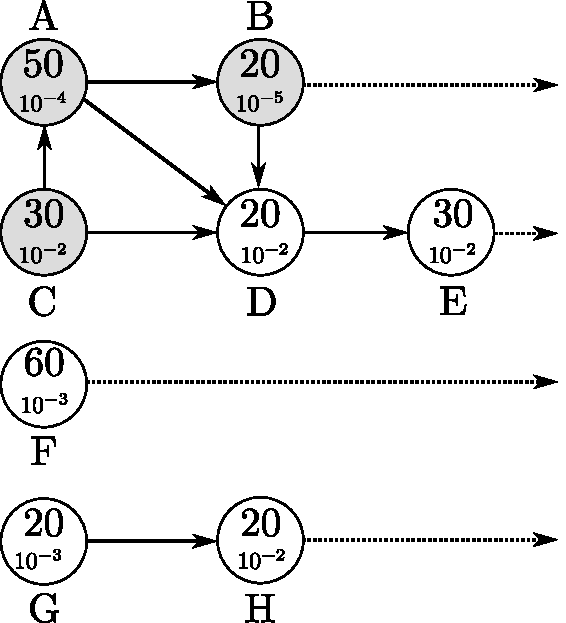
\includegraphics[width=3.5cm]{figs/avail_lo.pdf}}\quad
%		\raisebox{3em}{
%		\subfloat{
%			\includegraphics<3|handout:0>[width=5.5cm]{figs/fault_prop0.pdf}
%			\includegraphics<4|handout:0>[width=5.5cm]{figs/fault_prop1.pdf}
%			\includegraphics<5|handout:0>[width=5.5cm]{figs/fault_prop2.pdf}
%			\includegraphics<6>[width=5.5cm]{figs/fault_prop3.pdf}
%		}}
%	\end{figure}
%
%\end{frame}
%
%\begin{frame}
%	\frametitle{Availability enhancements: Fault propagation model}
%	\begin{equation}
%		A^{LO}_{i,k} = 1 - \left( p_i(LO) + 
%		\onslide<2->{\sum_{\color{red}\tau_j ~\in~
%		pred(\tau_i) ~\cup~ before_{HI}(j_{i,k})} p_j(LO)} \right).
%	\label{eq:avail_fp}
%	\end{equation}
%	
%	\begin{columns}
%		\begin{column}{.4\textwidth}
%			\begin{figure}
%				\vspace{-0.5cm}
%				\includegraphics<1-2|handout:0>[width=3.5cm]{figs/avail_lo.pdf}
%				\includegraphics<3->[width=3.5cm]{figs/avail_lo_fp.pdf}
%			\end{figure}
%		\end{column}
%		\begin{column}{.6\textwidth}
%			\begin{table}[]	
%				\centering
%				\begin{tabular}{c|c|c|}
%					\cline{2-3}
%					\multicolumn{1}{l|}{}                  & 
%					\multicolumn{2}{c|}{\textbf{Availability Rate}} \\ \hline
%					\multicolumn{1}{|c|}{\textbf{Outputs}} & Discard MC  & 
%					Enhanced  
%					\\ \hline
%					\multicolumn{1}{|c|}{\textit{E}}       & 95.78900\%    & 
%					\only{\textbf{\color{red}96.98900\%} }<3->  \\ \hline
%					\multicolumn{1}{|c|}{\textit{F}}       & 98.90000\%      & 
%					\only{98.90000\%}<4->   \\ \hline
%					\multicolumn{1}{|c|}{\textit{H}}       & 97.79000\%     & 
%					\only{\textbf{98.89000\%} }<4->    \\ \hline
%				\end{tabular}
%			\end{table}
%		\end{column}
%	\end{columns}
%	
%
%	
%	\begin{itemize}
%		\item<4-> Exact quantification with availability enhancements
%		$\rightarrow$ \textbf{Problem A2} $\checkmark$.
%	\end{itemize}
%\end{frame}
%
%
%
%\begin{frame}
%	\frametitle{Availability enhancements: Weakly-hard real-time tasks}
%	\begin{itemize}
%		\item Tolerate a number $m$ of faults for $k$ successive 
%		executions~\footfullcite{bernat2001weakly}.
%		\item Behavior of a $(1-2)$-firm WHRT task:
%	\end{itemize}
%	
%	\begin{figure}
%			\subfloat{
%				\includegraphics<1|handout:0>[width=5cm]{figs/time_empty.pdf}
%				\includegraphics<2|handout:0>[width=5cm]{figs/mkfirm_time0.pdf}
%				\includegraphics<3|handout:0>[width=5cm]{figs/mkfirm_time1.pdf}
%				\includegraphics<4|handout:0>[width=5cm]{figs/mkfirm_time2.pdf}
%				\includegraphics<5->[width=5cm]{figs/mkfirm_time3.pdf}
%			}\quad
%			\subfloat{\includegraphics<6->[width=4.5cm]{figs/mkfirm.pdf}}
%	\end{figure}
%	
%	\begin{itemize}
%		\item<7-> \emph{Limitation}: Exact availability quantification is no 
%		longer applicable.
%	\end{itemize}
%
%\end{frame}
%
%
%%------------------------------------------------------------------------------
%\section {System simulations}
%%------------------------------------------------------------------------------
%
%\begin{frame}
%	\frametitle{System simulations: probabilistic automata}
%	\centering
%	\textbf{Problem:} Current state of the system dependent on previous 
%	executions $\rightarrow$ memorize previous states.
%	\begin{itemize}
%		\item<2-> \textbf{Solution}: Translation rules to PRISM automata 
%		(PA)~\footfullcite{KNP11}.
%		\begin{itemize}
%			\item<3-> \textit{Challenge 1}: scalability.
%			\item<3-> \textit{Challenge 2}: automation.
%
%		\end{itemize}
%
%	\end{itemize}
%	\setcounter{subfigure}{0}
%	\begin{figure}
%		\vspace{-0.7cm}
%		\subfloat{
%			\includegraphics<4->[width=3.5cm]{figs/mk_r1.pdf}
%			\label{subfig:prism_r1}
%		}
%		\subfloat{
%			\includegraphics<4->[width=3.5cm]{figs/mk_r2.pdf}
%			\label{subfig:prism_r2}
%		}
%		\subfloat{
%			\includegraphics<4->[width=3.5cm]{figs/mk_r3.pdf}
%			\label{subfig:prism_r3}
%		}
%		\label{fig:prism_rules}
%	\end{figure}
%\end{frame}
%
%%------------------------------------------------------------------------------
%
%\begin{frame}
%	\frametitle{System simulations: results}
%	
%	\begin{figure}
%		\subfloat[WHRT rule]{
%			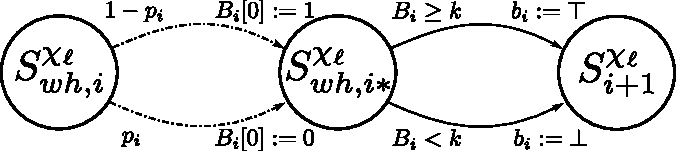
\includegraphics[width=7cm]{figs/mk_r4.pdf}
%			\label{subfig:prism_r4}
%		}
%	\end{figure}
%
%	\begin{table}[]	
%		\centering
%		\begin{tabular}{c|c|c|c|}
%			\cline{2-4}
%			\multicolumn{1}{l|}{}                  & 
%			\multicolumn{3}{c|}{\textbf{Availability Rate}} \\ \hline
%			\multicolumn{1}{|c|}{\textbf{Outputs}} & Discard MC  & Enhanced FP  
%			& 
%			Enhanced FP + WHRT \\ \hline
%			\multicolumn{1}{|c|}{\textit{E}}       & 95.78900\%    & 
%			96.98900\%     
%			&       \only{\textbf{97.90121\%}}<2->       \\ \hline
%			\multicolumn{1}{|c|}{\textit{F}}       & 98.90000\%      & 
%			98.90000\%       & 
%			\only{98.90099\%}<2->             \\ \hline
%			\multicolumn{1}{|c|}{\textit{H}}       & 97.79000\%     & 
%			98.89000\%      & \only{98.89441\%}<2->         \\ \hline
%		\end{tabular}
%		\label{tab:avail_enhance}
%	\end{table}
%	\begin{itemize}
%		\item<2-> Evaluation framework for state-dependent execution model 
%		$\rightarrow$ \textbf{Problem A3} $\checkmark$.
%		\item<2-> Translation rules integrated into the MC-DAG framework.
%	\end{itemize}
%\end{frame}
%
%%------------------------------------------------------------------------------
%%\subsection {Conclusion on availability analysis}
%%------------------------------------------------------------------------------
%
%\begin{frame}
%	\frametitle{Conclusion on availability analysis of MCS}
%	
%	\begin{itemize}
%		\item First contributions quantifying availability.
%		\item Exact method.
%		\begin{itemize}
%			\item Fault model and recovery mechanism.
%			\item Fault propagation mechanism to improve availability.
%		\end{itemize}
%		\item Simulations estimation for state-dependent execution model.
%		\begin{itemize}
%			\item Defined translation rules to obtain PA.
%
%		\end{itemize}
%		\item Evaluation framework compatible with our scheduling contributions.
%		\item Deliver min. service possible with discard MC model.
%	\end{itemize}
%\end{frame}
%
%%------------------------------------------------------------------------------
%\part{Conclusions and research perspectives}
%%------------------------------------------------------------------------------
%
%\miniframeson
%
%%------------------------------------------------------------------------------
%\section{Conclusions}
%%------------------------------------------------------------------------------
%
%\begin{frame}
%	\frametitle{Conclusions}
%	
%	\begin{block}{Efficient multi-periodic MC-DAG scheduling on multi-cores}
%		\begin{itemize}
%			\item Defined a general property to have safe mode transitions.
%			\item Proposed a generic meta-heuristic.
%			\item Implementations outperform state-of-the-art + good 
%			schedulability. 
%		\end{itemize}
%	\end{block}
%
%	\begin{block}{Guaranteed availability for MCS}<2>
%		\begin{itemize}
%			\item First quantification of availability for MCS.
%			\item Evaluation framework proved that availability enhancements 
%			are efficient.
%		\end{itemize}
%	\end{block}
%\end{frame}
%
%%------------------------------------------------------------------------------
%\section{Perspectives}
%%------------------------------------------------------------------------------
%
%\begin{frame}
%	\frametitle{Perspectives}
%	\begin{block}{Extensions to the MC-DAG model}
%		\begin{itemize}
%			\item Define other communication model.
%			\begin{itemize}
%				\item \emph{E.g.} Vertices sampled at different rates on 
%				reactive systems.
%			\end{itemize}
%			\item Incorporate elastic MC-tasks as vertices.
%		\end{itemize}
%	\end{block}
%
%	\begin{block}{System design trade-offs}
%		\begin{itemize}
%			\item Availability vs. schedulability.
%			\begin{itemize}
%				\item Reach availability rate and keep feasible schedules.
%			\end{itemize}
%			\item Availability-aware \textsc{Mh-McDag} implementation.
%		\end{itemize}
%	\end{block}
%\end{frame}
%
%
%\miniframesoff
%
%\begin{frame}[plain,noframenumbering]
%\frametitle{List of publications}
%
%\setbeamerfont{bibliography item}{size=\footnotesize}
%\setbeamerfont{bibliography entry author}{size=\footnotesize}
%\setbeamerfont{bibliography entry title}{size=\footnotesize}
%\setbeamerfont{bibliography entry location}{size=\footnotesize}
%\setbeamerfont{bibliography entry note}{size=\footnotesize}
%\begin{thebibliography}{1}
%	
%	\beamertemplatearticlebibitems
%	\bibitem{2018scheduling}
%	Roberto Medina, Etienne Borde and Laurent Pautet
%	\newblock Scheduling Multi-Periodic Mixed-Criticality DAGs on Multi-core 
%	Architectures
%	\newblock 39th IEEE Real-Time Systems Symposium (RTSS), 2018.
%	
%	\beamertemplatearticlebibitems
%	\bibitem{2018availability}
%	Roberto Medina, Etienne Borde and Laurent Pautet
%	\newblock {Availability Enhancement and Analysis for Mixed-Criticality 
%		Systems on Multi-Core}.
%	\newblock Design, Automation and Test in Europe (DATE) Conference and 
%	Exhibition, 2018. IEEE.
%	
%	\beamertemplatearticlebibitems
%	\bibitem{2017acyclic}
%	Roberto Medina, Etienne Borde and Laurent Pautet
%	\newblock {Directed Acyclic Graph Scheduling for Mixed-Criticality 
%		Systems}.
%	\newblock Ada-Europe International Conference on Reliable Software 
%	Technologies, 2017.
%	
%	\beamertemplatearticlebibitems
%	\bibitem{2016avail}
%	Roberto Medina, Etienne Borde and Laurent Pautet
%	\newblock {Availability analysis for synchronous data-flow graphs in 
%		mixed-criticality systems}.
%	\newblock 11th IEEE Symposium on Industrial Embedded Systems (SIES), 2016.
%	
%\end{thebibliography}
%\end{frame}
%
%%------------------------------------------------------------------------------
%
%\begin{frame}[plain,noframenumbering]
%
%	\frametitle{Conclusions}
%		\begin{block}{Efficient multi-periodic MC-DAG scheduling on multi-cores}
%		\begin{itemize}
%			\item Defined a general property to have safe mode transitions.
%			\item Proposed a generic meta-heuristic.
%			\item Implementations outperform state-of-the-art + good 
%			schedulability. 
%		\end{itemize}
%	\end{block}
%	
%	\begin{block}{Guaranteed availability for MCS}
%		\begin{itemize}
%			\item First quantification of availability for MCS.
%			\item Evaluation framework proved that availability enhancements 
%			are efficient.
%		\end{itemize}
%	\end{block}
%\end{frame}

\end{document}
